%%%% -*- Mode: LaTeX -*-
\documentclass[a4paper,12pt,openany,oneside]{book}
\usepackage{geometry}
 \geometry{
 	a4paper,
 	left=25mm,
 	top=30mm,
 	bottom=40mm,
 	right=25mm
 }
\usepackage[T1]{fontenc}
\usepackage[utf8]{inputenc}
\usepackage[italian]{babel}

% Packages AMS
\usepackage{amsmath}
\usepackage{amsfonts}
\usepackage{listings}
\usepackage{amssymb}
\usepackage{amsthm}
\usepackage{url}
% Simboli matematici aggiuntivi
\usepackage{stmaryrd}
\usepackage{verbatim}
% Per creare l'indice
\usepackage{index}
% Per spazi dopo le macro
\usepackage{xspace}
% Importazioni e manipolazione di grafica
\usepackage{graphicx}
% Per \begin{comment} ... \end{comment}
\usepackage{comment}
% Per la spaziatura tra linee
\usepackage{setspace}
% Per una migliore resa tipografica con pdflatex
\usepackage{microtype}

\usepackage{booktabs}
\usepackage{tabularx}
\usepackage{float}
\usepackage[final]{pdfpages}
\usepackage{geometry}
\usepackage{caption}
\usepackage[hidelinks]{hyperref}
\usepackage{float}
\restylefloat{table}
\usepackage{helvet}
\newcommand{\myparagraph}[1]{\paragraph{#1}\mbox{}\\[0.8em]}


\renewcommand{\familydefault}{\sfdefault}

\onehalfspacing



\title{Progetto Data Technology e Machine Learning}
\author{Matteo Colella, Matteo Angelo Costantini, Dario Gerosa}
\date{13/02/2018}

\makeindex

\begin{document}
%\fontencoding{T1}
%\fontfamily{palatino}
%\fontseries{m}
%\fontshape{it}
%\fontsize{12}{15}
\selectfont
\maketitle

\tableofcontents

\chapter{Introduzione}
In questo elaborato verrà mostrato il processo di integrazione di tre dataset appartenenti allo stesso dominio applicativo in modo da generare un terzo dataset a partire dal quale verranno applicate delle tecniche di clustering tramite l'algoritmo \textit{K-Means} al fine di evidenziare delle strutture intrinseche presenti nei dati.
I dataset utilizzati riguardano i risultati di 50 000 partite al videogioco competitivo \textit{DOTA 2}.
\\[0.8em]
\textit{DOTA 2} è un videogame in cui due squadre di cinque giocatori ciascuna si scontrano con l'obiettivo di distruggere le torri della squadra avversaria e infine la base nemica. All'inizio di una partita ogni giocatore deve scegliere un \textit{champion} (personaggio) da utilizzare per tutta la durata della partita. Ogni campione ha delle abilità e statistiche che lo caratterizzano e, per poter vincere, i giocatori devono cercare di scegliere i campioni in modo da andare a comporre una squadra il più equilibrata possibile.
\\[0.8em]
Il dataset principale contiene una tupla per ogni giocatore e per ogni partita per un totale di 500 000 tuple e 71 attributi riguardanti le performace del giocatore. Il secondo dataset contiene 50 000 tuple, una per ogni partita giocata, e 14 attributi tra cui la durata della partita e la squadra vincitrice. Infine, il terzo dataset contiene i 110 nomi dei personaggi del videogame associati ai loro rispettivi identificatori.
\\[0.8em]
La relazione è suddivisa in due parti. Nel capitolo relativo a Data Technology vengono analizzati i dataset utilizzati e verranno valutate due dimensioni di qualità; successivamente viene descritto dettagliatamente il processo di integrazione dei tre dataset, verranno analizzati i dataset ottenuti alla fine del processo, verranno ricalcolate le due dimensioni di qualità già calcolate in precedenza evidenziandone le differenze rispetto alle stesse prima del processo di integrazione; infine verranno effettuate delle analisi descrittive sui dataset (prima e dopo l'integrazione). Nel capitolo relativo a Machine Learning, dopo aver presentato il problema, vengono analizzate le feature del dataset evidenziandone in particolare le correlazioni al fine di scegliere le feature più importanti; successivamente vengono descritti i quattro esperimento condotti sui dataset integrati e verranno analizzati i risultati ottenuti; infine l'ultima sezione viene dedicata alle conclusioni.

\chapter{Data Technology}
I dataset iniziali sono stati reperiti da \url{kaggle.com} e sono stati costruiti sfruttando le API offerte dalla piattaforma \textit{Steam}, sviluppatrice del videogioco. Tramite questa API è possibile scaricare informazioni riguardanti un match conoscendone l'id. A causa delle limitazioni delle API non è però possibile ottenere gli id di match con certe caratteristiche (ad esempio tutti i match giocati in una cerca giornata, o quelli riguardanti un certo livello dei giocatori), ma si può solo visitare il grafo dei giocatori, ottenendo gli id delle partite che hanno giocato e gli id dei giocatori nella stessa partita. Questo porta sicuramente ad uno sbilanciamento del dataset limitando le informazioni a partite relative a giocatori con lo stesso livello di abilità.
\\[0.8em]
I dataset scelti per l'integrazione sono tre e tutti in formato csv, per questo motivo abbiamo deciso di rappresentarli attraverso un modello relazionale. Per la manipolazione abbiamo deciso di utilizzare il DBMS \verb|SQLite| e la libreria \verb|pandas| di Python. In particolare abbiamo deciso di utilizzare \verb|SQLite| in quanto per le necessità del progetto e per la mole contenuta di dati da manipolare abbiamo ritenuto che sarebbe stato troppo dispendioso in termini di tempo l'utilizzo di altri DBMS più completi (Postgres, MySQL\dots) per avere minimi vantaggi in termini prestazionili. Infatti, il DBMS è stato utilizzato solo a fini esplorativi ed è risultati comunque estremamente veloce sia nell'importazioni che nelle query. Tutto il lavoro di integrazione è stato invece svolto utilizzando \verb|pandas|.
\section{Descrizione dei dataset}
\subsection{Dataset matches}\label{subsection:matches}
Questo è il dataset principale contenente 500 000 istanze. Ogni istanza contiene informazioni relative alle performance di un \textit{champion} in uno specifico \textit{match}. Gli attributi inizialmente presenti in questo dataset sono 71, per praticità elenchiamo di seguito solo quelli di interesse, ovvero gli attributi rimasti dopo la prima fase di integrazione descritta successivamente.
\begin{itemize}
	\item match\_id	: l'identificatore della partita;
	\item player\_slot : l'identificatore del giocatore all'interno della partita. I giocatori della squadra \textit{Radiant} hanno valori che vanno da 0 a 4, mentre i giocatori della squadra \textit{Dire} hanno valori che vanno da 128 a 132.
	\item hero\_id : l'identificatore del \textit{champion};
	\item gold : l'ammontare delle monete del giocatore alla fine della partita;
	\item gold\_spent : l'ammontare delle monete spese durante la partita;
	\item xp\_creep : l'esperienza guadagnata dal giocatore uccidendo i \textit{creep};
	\item xp\_hero : l'esperienza base guadagnata dal giocatore;
	\item xp\_roshan : l'esperienza guadagnata dal \textit{Roshan The Immortal};
	\item xp\_other : l'esperienza guadagnata in altri modi;
	\item kills : numero di uccisioni in quella partita;
	\item deaths : numero di morti del giocatore in quella partita;
	\item assists : numero di partecipazioni alle uccisioni; 
	\item lasthits : numero di \textit{creep} uccisi;
	\item hero\_damage : danno inflitto dal giocatore;
	\item hero\_healing : danni curati dal giocatore;
	\item tower\_damage : danni inflitti alle torri;
\end{itemize}
\begin{table}[ht]
	\scriptsize	
	\centering	
			\begin{tabularx}{0.82\textwidth}{rrrrrrrrr}
                match\_id & player\_slot & hero\_id & gold & gold\_spent & xp\_creep & xp\_hero & xp\_roshan & \dots \\
                \midrule                                                                
                0     &       0    &   86 & 3261   &    10960  &  5440.0 &  8840.0   &     NaN               & \dots \\
                0     &      1    &   51 & 2954   &    17760  &  8440.0 & 14331.0  &   2683.0                & \dots \\
                0     &       2    &   83  & 110    &   12195  &  8112.0  & 6692.0    &    NaN               & \dots \\
                0     &       3    &   11 & 1179    &   22505  & 14230.0 &  8583.0   &   894.0               & \dots \\
                0     &      4   &    67 & 3307   &    23825 &  14325.0 & 15814.0    &    NaN                & \dots \\
                0     &     128  &   106 &  476   &    12285 &  12259.0 &  8502.0    &    NaN                & \dots \\
                0     &     129  &    102 &   317   &    10355  &  9417.0 &  5201.0   &     NaN              & \dots \\
                0     &     130  &     46 & 2390    &   13395 &  13396.0 &  6853.0    &    NaN               & \dots \\
                0     &     131  &      7 &  475    &    5035  &  4038.0 &  4798.0    &    NaN               & \dots \\
                0     &     132  &     73  &  60    &   17550  & 10471.0 &  6659.0 & NaN                          & \dots 
			\end{tabularx}
			\\[3.0em]
			\begin{tabularx}{0.855\textwidth}{rrrrrrrrr}
                \dots & xp\_other & kills & deaths & assists & last\_hits & hero\_damage & hero\_healing & tower\_damage \\
                \midrule
                \dots &  83.0   &   9   &    3   &    18    &     30    &     8690     &      218       &    143  \\
                \dots &  671.0   &  13   &    3   &    18    &    109    &    23747     &        0       &    423  \\
                \dots &  453.0   &   0   &    4   &    15    &     58    &     4217     &     1595       &    399  \\
                \dots &  293.0   &   8   &    4   &    19    &    271    &    14832     &     2714       &   6055  \\
                \dots &  62.0   &  20   &    3   &    17    &    245    &    33740     &      243       &   1833  \\
                \dots &  1.0   &   5   &    6   &     8    &    162    &    10725     &        0       &    112  \\
                \dots &  1.0   &   4   &   13   &     5    &    107    &    15028     &      764       &      0  \\
                \dots &  244.0   &   4   &    8   &     6    &    208    &    10230     &        0       &   2438  \\
                \dots &  27.0   &   1   &   14   &     8    &     27    &     4774     &        0       &      0  \\
                \dots &  933.0   &   1   &   11   &     6    &    147    &     6398     &      292       &      0  \\
			\end{tabularx}
			\captionof{table}{dataset matches}
			\label{table:matches}
\end{table}

\subsection{Dataset matches\_stats}
Questo dataset contiene per ogni \textit{match} la sua durata e la squadra vincitrice. In particolare utilizziamo il primo attributo per calcolare delle feature in relazione al tempo giocato. Mentre il secondo viene utilizzato per calcolare la percentuale di vittoria di ogni campione. Come per la tabella precedente, anche in questo caso vengono riportati solo gli attributi di interesse. Sono quindi stati omessi 14 attributi.
\begin{table}[ht]
	\scriptsize	
	\centering	
	\begin{tabularx}{0.3\textwidth}{rrl}
		match\_id & duration & radiant\_win \\
		\midrule
		0 &     2375 &        True \\
		1 &     2582 &       False \\
		2 &     2716 &       False \\
		3 &     3085 &       False \\
		4 &     1887 &        True \\
		5 &     1574 &        True \\
		6 &     2124 &        True \\
		7 &     2328 &        True \\
		8 &     2002 &       False \\
		9 &     2961 &       False \\
	\end{tabularx}	
	\captionof{table}{dataset matches\_stats}
	\label{table:matches_stats}
\end{table}
\begin{itemize}
	\item match\_id : l'identificatore del match giocato;
	\item duration : la durata in secondi del match;
	\item radiant\_win : indica se la squadra \textit{radiant} ha vinto o meno la partita.
\end{itemize}

\subsection{Dataset hero\_names}
Questo dataset associa ad ogni identificatore numerico del campione sia il suo nome in inglese sia un identificatore leggibile. Utilizziamo questo dataset per associare il nome del campione ad ogni istanza del dataset principale.
\begin{table}[ht]
	\scriptsize	
	\centering	
	\begin{tabularx}{0.5\textwidth}{lrl}
        name & hero\_id & localized\_name \\
        \midrule
        npc\_dota\_hero\_antimage &       1 &      Anti-Mage \\
        npc\_dota\_hero\_axe &       2 &            Axe \\
        npc\_dota\_hero\_bane &       3 &           Bane \\
        npc\_dota\_hero\_bloodseeker &       4 &    Bloodseeker \\
        npc\_dota\_hero\_crystal\_maiden &       5 & Crystal Maiden \\
        npc\_dota\_hero\_drow\_ranger &       6 &    Drow Ranger \\
        npc\_dota\_hero\_earthshaker &       7 &    Earthshaker \\
        npc\_dota\_hero\_juggernaut &       8 &     Juggernaut \\
        npc\_dota\_hero\_mirana &       9 &         Mirana \\
        npc\_dota\_hero\_morphling &      10 &      Morphling \\
	\end{tabularx}
	\captionof{table}{dataset hero\_names}
\end{table}
\begin{itemize}
	\item name: identificatore testuale del campione;
	\item hero\_id: identificatore numerico;
	\item localized\_name: nome in inglese;
\end{itemize}

\section{Analisi di dimensioni di qualità (prima dell'integrazione)}
Sono state effettute le seguenti due misure di qualità:
\begin{itemize}
	\item Completezza
	\item Consistenza
\end{itemize}
Di seguito verranno descritti i passi svolti per l'analisi delle due misure in relazione ai dataset iniziali.
\subsection{Completezza}\label{subsection:completezza1}
Per valutare la completezza dei dataset di partenza abbiamo calcolato le percentuali di valori nulli per ogni attributo del dataset, per ogni tupla e sul totale di valori per ognuno dei dataset di partenza. Tutte le operazioni sono state svolte utilizzando la libreria \verb|pandas| di Python. Di seguito i valori riportati per ogni tabella.

\begin{table}[H]
	\tiny	
	\centering	
	\begin{tabularx}{0.37\textwidth}{lrr} 
		attribute                           &   \# NaN    &   \% NaN              \\
		\midrule
		match\_id                            &   0             &   0.0                    \\
		account\_id                          &   0             &   0.0                    \\
		hero\_id                             &   0             &   0.0                    \\
		player\_slot                         &   0             &   0.0                    \\
		gold                                &   0             &   0.0                    \\
		gold\_spent                          &   0             &   0.0                    \\
		kills                               &   0             &   0.0                    \\
		deaths                              &   0             &   0.0                    \\
		assists                             &   0             &   0.0                    \\
		denies                              &   0             &   0.0                    \\
		last\_hits                           &   0             &   0.0                    \\
		stuns                               &   0             &   0.0                    \\
		hero\_damage                         &   0             &   0.0                    \\
		hero\_healing                        &   0             &   0.0                    \\
		tower\_damage                        &   0             &   0.0                    \\
		item\_0                              &   0             &   0.0                    \\
		item\_1                              &   0             &   0.0                    \\
		item\_2                              &   0             &   0.0                    \\
		item\_3                              &   0             &   0.0                    \\
		item\_4                              &   0             &   0.0                    \\
		item\_5                              &   0             &   0.0                    \\
		level                               &   0             &   0.0                    \\
		leaver\_status                       &   0             &   0.0                    \\
		xp\_hero                             &   1883          &   0.38                 \\
		xp\_creep                            &   68            &   0.01                 \\
		xp\_roshan                           &   320438        &   64.00                \\
		xp\_other                            &   21036         &   4.21                 \\
		gold\_other                          &   94897         &   18.98                \\
		gold\_death                          &   6299          &   1.26                 \\
		gold\_buyback                        &   352859        &   70.57                \\
		gold\_abandon                        &   479366        &   95.87                \\
		gold\_sell                           &   102593        &   20.52                \\
		gold\_destroying\_structure           &   19675         &   3.94     \\
		gold\_killing\_heros                  &   1565          &   0.31                  \\
		gold\_killing\_creeps                 &   294           &   0.059                 \\
		gold\_killing\_roshan                 &   240264        &   48.05                \\
		gold\_killing\_couriers               &   403021        &   80.60                \\
		unit\_order\_none                     &   499994        &   99.99                \\
		unit\_order\_move\_to\_position         &   42            &   0.01                 \\
		unit\_order\_move\_to\_target           &   54550         &   10.91                  \\
		unit\_order\_attack\_move              &   113271        &   22.65                \\
		unit\_order\_attack\_target            &   105           &   0.02                  \\
		unit\_order\_cast\_position            &   2269          &   0.45    \\
		unit\_order\_cast\_target              &   16674         &   3.33     \\
		unit\_order\_cast\_target\_tree         &   35712         &   7.14                 \\
		unit\_order\_cast\_no\_target           &   892           &   0.18                 \\
		unit\_order\_cast\_toggle              &   401211        &   80.24                \\
		unit\_order\_hold\_position            &   137277        &   27.46                \\
		unit\_order\_train\_ability            &   73            &   0.01                 \\
		unit\_order\_drop\_item                &   288667        &   57.73                \\
		unit\_order\_give\_item                &   394631        &   78.93      \\
		unit\_order\_pickup\_item              &   244658        &   48.93     \\
		unit\_order\_pickup\_rune              &   74517         &   14.90                \\
		unit\_order\_purchase\_item            &   57            &   0.01                 \\
		unit\_order\_sell\_item                &   111866        &   22.37     \\
		unit\_order\_disassemble\_item         &   485446        &   97.09      \\
		unit\_order\_move\_item                &   4264          &   0.85     \\
		unit\_order\_cast\_toggle\_auto         &   463670        &   92.73      \\
		unit\_order\_stop                     &   412425        &   82.49                 \\
		unit\_order\_taunt                    &   500000        &   100.0                  \\
		unit\_order\_buyback                  &   352233        &   70.45                \\
		unit\_order\_glyph                    &   273230        &   54.65     \\
		unit\_order\_eject\_item\_from\_stash    &   468736        &   93.75      \\
		unit\_order\_cast\_rune                &   499991        &   99.99                \\
		unit\_order\_ping\_ability             &   160852        &   32.17                \\
		unit\_order\_move\_to\_direction        &   496449        &   99.29                \\
		unit\_order\_patrol                   &   500000        &   100.0                  \\
		unit\_order\_vector\_target\_position   &   500000        &   100.0                  \\
		unit\_order\_radar                    &   500000        &   100.0                  \\
		unit\_order\_set\_item\_combine\_lock    &   500000        &   100.0                  \\
		unit\_order\_continue                 &   500000        &   100.0                  \\
	\end{tabularx}
	\captionof{table}{Completezza di matches}
\end{table}
\myparagraph{matches}
\textit{Completezza della tabella:}\\
\begin{itemize}
	\item Numero di tuple: 500 000
	\item Numero di attributi: 71
	\item Numero di valori null: 11 038 020
	\item Numero di valori della tabella: 35 500 000
	\item Completezza tabella: 68,91\%
	\item Completezza tabella utilizzata: 95,07\%
\end{itemize}
\begin{table}[htb]
	\tiny	
	\centering	
	\begin{tabularx}{0.25\textwidth}{lrr} 
		Attributo     &    \# NaN  &    \% NaN \\
		\midrule
		match\_id      &        0   &    0.00 \\
		player\_slot   &        0   &    0.00 \\
		hero\_id       &        0   &    0.00 \\
		gold          &        0   &    0.00 \\
		gold\_spent    &        0   &    0.00 \\
		xp\_creep      &       68   &    0.01 \\
		xp\_hero       &     1883   &    0.38 \\
		xp\_roshan     &   320438   &   64.09 \\
		xp\_other      &    21036   &    4.21 \\
		kills         &        0   &    0.00 \\
		deaths        &        0   &    0.00 \\
		assists       &        0   &    0.00 \\
		last\_hits     &        0   &    0.00 \\
		hero\_damage   &        0   &    0.00 \\
		hero\_healing  &        0   &    0.00 \\
		tower\_damage  &        0   &    0.00 \\
	\end{tabularx}
	\captionof{table}{Completezza di matches ridotta ai soli attributi di interesse}
	\label{tab:comp_matches}
\end{table}
\myparagraph{heroes\_names}
\begin{table}[H]	
	\centering	
	\begin{tabularx}{0.30\textwidth}{lr} 
		Attributo    &   \# NaN \\
		\midrule
		name            &  0 \\
		hero\_id         &  0 \\
		localized\_name  &  0 \\
	\end{tabularx}
	\captionof{table}{Completezza di heroes\_names}		
\end{table}
\noindent
\myparagraph{matches\_stats}
\begin{table}[H]	
	\centering	
	\begin{tabularx}{0.40\textwidth}{lr} 
		attributo  & \# NaN \\
		\midrule
		match\_id                 &  0 \\
		start\_time               &  0 \\
		duration                 &  0 \\
		tower\_status\_radiant     &  0 \\
		tower\_status\_dire        &  0 \\
		barracks\_status\_dire     &  0 \\
		barracks\_status\_radiant  &  0 \\
		first\_blood\_time         &  0 \\
		game\_mode                &  0 \\
		radiant\_win              &  0 \\
		negative\_votes           &  0 \\
		positive\_votes           &  0 \\
		cluster                  &  0 \\
	\end{tabularx}
	\captionof{table}{Completezza di matches\_stats}
\end{table}

\myparagraph{Osservazioni}
Come si può notare sono presenti un gran numero di attributi con valore nulla, ma se restringiamo il campio ai soli attributi di nostro interesse (quelli mostratai in tabella \ref{table:matches}) il numero di valori null dimunisce sensibilemente e il contributo maggiore è dovuto ai valori mancanti per l'attributo \verb|xp_roshan| che contribuisce per il 64\% dei null di tutta la tabella. Un'altra osservazione che abbiamo potuto fare è relativa alla natura di questi valori: abbiamo infatti notato che le API utilizzate non includevano gli attributi relativi all'esperienza ottenuta qualora il suo valore fosse stato 0 e che quindi tutti i valori null sono in realtà 0. Questa ipotesi è anche confermata dal fatto che, per ognuno dei quattro attributi, non sono presenti valori pari a 0 in tutto il dataset. Per questo motivo abbiamo deciso di correggere i valori mancanti assegnandogli 0 durante la fase di integrazione dei dataset.

\subsection{Consistenza}
Durante il processo di integrazione ci siamo accorti che dopo aver effettuato la join tra il dataset \verb|heroes_names| contenente il nome dei campioni con il dataset dei match, ottenevamo solo 499 963 match anziché 500 000 a causa di una discrepanza tra gli id dei campioni contenuti in \verb|heroes_names| e quelli contenuti in \verb|matches|. Indagando ulteriormente abbiamo notato che per quanto riguarda la prima tabella il range dei valori variava tra 1 e 113, mentre nella seconda tabella tra 0 e 112. Inizialmente questo ci ha portato ha pensare che gli id fossero semplicemente shiftati di un valore. Per confermare quest'ipotesi abbiamo quindi provato ad effettuare una join incrementando di uno il valore degli id della tabella \verb|heroes_stats|. Il risultato della join è stato però differente da quanto ci aspettavamo, 482 312 corrispondenze, meno che nel caso precedente. Questo ha portato ad escludere l'ipotesi dello shift degli id. Analizzando ulteriormente i due dataset abbiamo notato che in entrambi i dataset non era mai presente l'id 24. Abbiamo quindi ipotizzato che l'eroe identificato con l'id 113 non sia presente nel dataset \verb|matches| perché il campione associato è stato rilasciato in un periodo successivo a quello di svolgimento dei match contenuti nel dataset. Analogamente, ipotizziamo che il campione con id 0 non sia presente nella tabella \verb|heroes_names| perché è stato rimosso dal gioco.

Non sono state quindi effettuate modifiche agli id ed abbiamo deciso di utilizzare i 499 963 match anziché 500 000 dato che il numero di tuple perse è irrisorio rispetto alla dimensione del dataset.

\section{Processo di integrazione}
Il processo di integrazione è stato effettuato importando i dataset in Python e utilizzando la libreria \verb|pandas| e si è suddiviso nelle seguenti fasi di integrazione:
\begin{enumerate}
	\item Eliminati alcuni attributi del dataset \verb|matches|.
	\item Eliminati alcuni attributi del dataset \verb|matches_stats|.
	\item Calcolate feature aggiuntive per il dataset \verb|matches| sfruttando le informazioni di \verb|matches_stats|.
	\item Rimossi dalla tabella \verb|matches| tutti gli attributi utilizzati per il calcolo delle feature del passo precedente.
	\item Aggiunti i nomi dei campioni nella tabella \verb|matches|.
	\item Raggruppamento per \textit{champion} dei dati di \verb|matches| in un nuovo dataset \verb|heroes_stats|.
	\item Normalizzazione delle features.
	\item Inversione dei valori relativi all'attributo \verb|deaths|.
\end{enumerate}

\paragraph{Fase 1:} Questa prima fase è stata eseguita subito dopo aver scaricato i dataset in modo da limitare la quantita' di dati da dover manipolare inutilmente. Le feature iniziali si possono trovare nella tabella \verb|matches| dei dataset di partenza e non le abbiamo elencate in questa relazione. Il risultato di questa fate è mostrato in tabella \ref{table:matches}.
\paragraph{Fase 2:} Analogamente alla fase precedente, abbiamo eliminato da \verb|matches_stats| tutte le feature che non intendiamo utilizzare nelle fasi successive. Anche queste feature si possono trovare nella rispettiva tabella nei dataset iniziali. Il risultato di questa fase è mostrato in tabella \ref{table:matches_stats}.
\paragraph{Fase 3:} In questa fase sono stati calcolati gli attributi \verb|gold_over_duration|, \verb|won|, \verb|xp_over_duration| e \verb|picks|. Il primo attributo indica il numero medio di monete guadagnate al secondo ed è stato calcolato dividendo la somma degli attributi \verb|gold| e \verb|gold_spent| per il numero di secondi del match (valore presente nella tabella \verb|matches_stats|). Il secondo attributo fa riferimento all'esperienza guadagna in gioco dal giocatore ed è stata calcolata in modo analogo all'attributo precendente: abbiamo sommato i valori di esperienza dei quattro attributi relativi (descritti nella sottosezione \ref{subsection:matches}) e li abbiamo divisi per la durata della partita. Infine abbiamo aggiunto un attributo che indica se il giocatore ha vinto o meno la partita. Per fare questo abbiamo utilizzato l'attributo \verb|radiant_win| del dataset \verb|matches_stats| per sapere se la squadra \textit{Radiant} ha vinto o meno la partita e abbiamo poi controllato la squadra di appartenza del giocatore (attributo \verb|player_slot| di \verb|matches|) per sapere se ha vinto o meno.
\paragraph{Fase 4:} In questa fase abbiamo rimosso tutti gli attributi intermedi utilizzati per calcolare le feature della \textit{Fase 3} e che non hanno più alcuna utilità.
\paragraph{Fase 5:} Dopo aver rimosso gli attributi inutili abbiamo effettuato una join tra la tabella \verb|matches| ottenuta al passo successivo con la tebella \verb|heroes_names| per aggiungere i nomi dei campioni al dataset principale. Abbiamo deciso di utilizzare i nomi locallizati in inglese e non gli identificatori testuali o numerici per riferirci al campione per una questione di praticità.
\paragraph{Fase 6:} Una volta ottenuti tutti gli attributi di interesse abbiamo raggruppato in base al campione le tuple di \verb|matches| e calcolato le statistiche medie degli attributi a disposizione per ogni campione ed è stato aggiunto l'attributo \verb|picks| ovvero la percentuale di volte in cui un certo campione viene scelto da un giocatore. In questo modo abbiamo creato il dataset \verb|heroes_stats|.
\paragraph{Fase 7:} A questo punto abbiamo deciso di nornalizzare le feature in modo da lavorare con attributi con valori nello stesso range.
\paragraph{Fase 8:} In quest'ultima fase abbiamo sostituito i valori dell'attributo \verb|deaths| con il valore ottenuto calcolando $1 - deaths $. Abbiamo preso questa decisione in quanto questo attributo è l'unico che a valori maggiori fa corrispondere una performance del campione minore. Per tutti gli altri attributi a valori più alti corrispondono prestazioni migliori.
\section{Descrizione dei dataset finali}
\subsection{Dataset matches\_stats}
Questo è il dataset principale dopo il processo di integrazione e contiene 499 963 match. Non è quello su cui verrà fatto Machine Learning, ma è quello che ha permesso di creare il dataset su cui faremo il clustering, ovvero \verb|heroes_stats_normalized|. Il dataset contiene 11 attributi, tra cui il nome del campione ed è riportato in tabella \ref{table:matches_final}. Gli attributi sono i seguenti:
\begin{itemize}
	\item hero\_name : il nome del campione;
	\item kills : numero di uccisioni in quella partita;
	\item deaths : numero di morti del giocatore in quella partita;
	\item assists : numero di partecipazioni alle uccisioni; 
	\item lasthits : numero di \textit{creep} uccisi;
	\item hero\_damage : danno inflitto dal giocatore;
	\item hero\_healing : danni curati dal giocatore;
	\item tower\_damage : danni inflitti alle torri;
	\item gold\_over\_duration : monete medie guadagnate al secondo;
	\item xp\_over\_duration : esperienza media guadagnata al secondo;
	\item won : il giocatore ha vinto la partita;
\end{itemize}
\begin{table}[ht]
	\scriptsize	
	\centering	
	\begin{tabularx}{0.6\textwidth}{lrrrrrr}
		hero\_name & kills & deaths & assists & last\_hits & hero\_damage & \dots \\
		\midrule
		Rubick &     9 &      3 &      18 &        30 &        8690 & \dots \\      
		Rubick &     4 &     14 &      15 &        42 &        9757 & \dots \\      
		Rubick &     2 &      4 &      18 &       143 &        8208 & \dots \\      
		Rubick &     4 &      7 &      16 &        20 &        6273 & \dots \\      
		Rubick &    14 &      7 &      23 &        66 &       17818 & \dots \\ 
	\end{tabularx}
	\\[3.0em]
	\centering
	\begin{tabularx}{0.72\textwidth}{rrrrlr}
		\dots & hero\_healing & tower\_damage & gold\_over\_duration & xp\_over\_duration &   won \\
		\midrule
		\dots & 218 &          143 &           5.987789 &         6.047579 &  True \\
		\dots & 325 &          280 &           3.200608 &         4.691658 & False \\
		\dots & 0 &          151 &           5.091923 &         7.961724 & False \\
		\dots & 0 &          309 &           5.391186 &         5.889596 &  True \\
		\dots & 0 &          403 &           7.090737 &        10.257404 &  True \\
	\end{tabularx}
	\captionof{table}{dataset matches\_stats}
	\label{table:matches_final}
\end{table}

\subsection{Dataset heroes\_stats}\label{subsection:heroes_stats}
Questo è il dataset ottenuto aggregando le informazioni di \verb|matches| e contiene le statistiche medie per ogni campione. Abbiamo utilizzato questo dataset per l'analisi descrittiva dei dati in quanto i valori non sono ancora stati normalizzati e rappresentano la media effettiva del rispettivo attributo. Il dataset contiene 13 attributi tra cui il nome del campione, ed è riportato in tabella \ref{table:heroes_stats}. Gli attributi sono i seguenti: 
\begin{itemize}
	\item hero\_name : il nome del campione;
	\item kills : numero medio di uccisioni del \textit{champion};
	\item deaths : numero medio di morti del \textit{champion};
	\item assists : numero medio di partecipazioni alle uccisioni; 
	\item lasthits : numero medio di \textit{creep} uccisi;
	\item hero\_damage : danno medio inflitto dal giocatore;
	\item hero\_healing : danni medio curati dal giocatore;
	\item tower\_damage : danni medi inflitti alle torri;
	\item gold\_over\_duration : monete medie guadagnate al secondo;
	\item xp\_over\_duration : esperienza media guadagnata al secondo;
	\item won\_perc : percentuale di partite vinte dal \textit{champion};
	\item lost\_perc : percentuale di partite perse dal \textit{champion};
	\item picks : percentuale di volte in cui il \textit{champion} è stato usato in una partita.
\end{itemize}
\begin{table}[H]
	\scriptsize	
	\centering	
	\begin{tabularx}{0.92\textwidth}{lrrrrrrc}
		hero\_name &    kills &   deaths &   assists &  last\_hits &  hero\_damage & hero\_healing & \dots \\
		\midrule
		Abaddon & 5.005740 & 6.278550 & 12.647432 &  84.188822 &             9660.720846  & 2242.337462 & \dots \\
		Alchemist & 6.679019 & 7.173369 & 11.647562 & 265.160847 &           14438.700906 & 10.312735   & \dots \\
		Ancient Apparition & 4.826151 & 7.492818 & 13.356286 &  48.930994 &  8888.788094  & 213.265956  & \dots \\
		Anti-Mage & 7.340996 & 5.449979 &  6.722222 & 298.673585 &           10162.878033 & 135.156769  & \dots \\
		Axe & 8.525321 & 9.365138 & 10.498153 & 136.269724 &                 11945.333188 & 14.217779   & \dots \\
		Bane & 4.766941 & 7.721112 & 11.811986 &  32.764591 &                7838.933803  & 167.141794  & \dots \\
		Batrider & 6.055977 & 8.263757 & 14.039848 & 103.942125 &            10802.548387 & 75.833966   & \dots \\
		Beastmaster & 5.455987 & 7.912768 & 13.011895 & 111.848533 &         10093.486122 & 123.457573  & \dots \\
		Bloodseeker & 9.657307 & 9.190122 &  9.746279 & 165.670162 &         13487.634641 & 740.771651  & \dots \\
		Bounty Hunter & 6.731047 & 8.261446 & 10.033417 &  40.083910 &       9326.336228  & 771.840130  & \dots \\
	\end{tabularx}
	\\[3.0em]
	\centering
	\begin{tabularx}{0.87\textwidth}{crrrrrr}
        \dots & tower\_damage & gold\_over\_duration & xp\_over\_duration &  won\_perc & lost\_perc & picks\\
        \midrule
        \dots &  1009.606949 &           5.819416 &         6.967741 & 30.543807 & 69.456193       & 0.662049 \\
        \dots &  2585.172758 &          11.168695 &         9.629661 & 27.089484 & 72.910516         & 1.964745 \\
        \dots &  298.453280 &           4.936875 &         5.418059 & 26.047683 & 73.952317        & 1.350700 \\
        \dots &  3081.401767 &           8.875521 &         9.685556 & 23.893146 & 76.106854        & 1.879339 \\
        \dots &  453.616605 &           5.989381 &         7.394753 & 22.647251 & 77.352749         & 0.920268 \\
        \dots &  381.018801 &           4.624201 &         5.624299 & 24.441833 & 75.558167        & 0.510638 \\
        \dots &  268.393738 &           5.581703 &         6.986072 & 21.726755 & 78.273245         & 0.210816 \\
        \dots &  1491.495638 &           5.975999 &         7.124649 & 26.804124 & 73.195876        & 0.252219 \\
        \dots &  1449.624831 &           6.830154 &         8.259095 & 23.815968 & 76.184032        & 0.591244 \\
        \dots &  430.565141 &           6.581745 &         6.141938 & 25.732372 & 74.267628        & 1.358701 \\
	\end{tabularx}
	\captionof{table}{dataset heroes\_stats}
	\label{table:heroes_stats}
\end{table}

\subsection{Dataset heroes\_stats\_normalized}
Questo è il dataset su cui abbiamo effettuato il clustering e contiene gli stessi attributi della tabella \verb|heroes_stats|, ma con i valori normalizzati. Il risultato è riportato in tabella \ref{table:heroes_stats_normalized}. Essendo gli attributi quelli del dataset precedente con i valori normalizzati, le descrizioni sono le stesse della sottosezione \ref{subsection:heroes_stats}.
\begin{table}[H]
	\scriptsize	
	\centering	
	\begin{tabularx}{0.88\textwidth}{lrrrrrrc}
	    hero\_name &    kills &   deaths &  assists & last\_hits & hero\_damage & hero\_healing & \dots \\
	    \midrule
	    Abaddon & 0.251889 & 0.806403 & 0.550658 &  0.203026 &    0.276095 &            0.444800 & \dots \\
	    Alchemist & 0.414291 & 0.618982 & 0.470296 &  0.875475 &    0.520827 &          0.001890 & \dots \\
	    Ancient Apparition & 0.234459 & 0.552074 & 0.607631 &  0.072017 &    0.236556 & 0.042163 & \dots \\
	    Anti-Mage & 0.478540 & 0.979947 & 0.074435 &  1.000000 &    0.301816 &          0.026664 & \dots \\
	    Axe & 0.593486 & 0.159916 & 0.377916 &  0.396546 &    0.393115 &                0.002665 & \dots \\
	    Bane & 0.228712 & 0.504257 & 0.483511 &  0.011946 &    0.182782 &               0.033010 & \dots \\
	    Batrider & 0.353821 & 0.390600 & 0.662570 &  0.276425 &    0.334581 &           0.014892 & \dots \\
	    Beastmaster & 0.295588 & 0.464115 & 0.579951 &  0.305803 &    0.298262 &        0.024342 & \dots \\
	    Bloodseeker & 0.703352 & 0.196573 & 0.317486 &  0.505791 &    0.472113 &        0.146838 & \dots \\
	    Bounty Hunter & 0.419340 & 0.391084 & 0.340564 &  0.039143 &    0.258968 &      0.153003 & \dots \\
	\end{tabularx}
	\\[3.0em]
	\centering
	\begin{tabularx}{0.83\textwidth}{crrrrrr}
	    \dots & tower\_damage & gold\_over\_duration & xp\_over\_duration & won\_perc & lost\_perc & picks \\
	    \midrule
	    \dots &     0.225532 &           0.207991 &         0.298929 & 0.914078 &  0.085922 & 0.134519 \\
	    \dots &     0.661543 &           1.000000 &         0.732669 & 0.613589 &  0.386411 & 0.455325 \\
	    \dots &     0.028733 &           0.077323 &         0.046419 & 0.522963 &  0.477037 & 0.304108 \\
	    \dots &     0.798866 &           0.660475 &         0.741777 & 0.335541 &  0.664459 & 0.434292 \\
	    \dots &     0.071671 &           0.233156 &         0.368507 & 0.227161 &  0.772839 & 0.198109 \\
	    \dots &     0.051581 &           0.031028 &         0.080025 & 0.383271 &  0.616729 & 0.097232 \\
	    \dots &     0.020414 &           0.172795 &         0.301915 & 0.147088 &  0.852912 & 0.023397 \\
	    \dots &     0.358887 &           0.231174 &         0.324496 & 0.588765 &  0.411235 & 0.033593 \\
	    \dots &     0.347300 &           0.357640 &         0.509345 & 0.328827 &  0.671173 & 0.117082 \\
	    \dots &     0.065292 &           0.320860 &         0.164370 & 0.495534 &  0.504466 & 0.306078 \\
	\end{tabularx}
	\captionof{table}{dataset heroes\_stats\_normalized}
	\label{table:heroes_stats_normalized}
\end{table}
\section{Analisi di dimensioni di qualità (dopo l'integrazione)}
Dopo il processo di integrazione le misure di completezza e consistenza risultano perfette al 100\%. Infatti, come descritto nella sezione \ref{subsection:completezza1}, dopo aver valutato la natura dei valori null presenti nella tabella, abbiamo deciso di sostituirli con il valore 0 e quindi siamo riusciti ad ottenere una completezza totale della tabella. Tutti gli attributi calcolati successivamente, durante il processo di integrazione, utilizzavano quindi le informazione di dataset completi ed è stato dunque possibile calcolarne il valore per ogni tupla.
\\
Per quanto riguarda la consistenza, dopo aver eliminato le tuple di \verb|matches| contenenti un eroe non disponibile nella tabella \verb|heroes_names| abbiamo portato la consistenza al 100\% e da quel momento non abbiamo introdotto modifiche agli identificatori e le uniche modifiche alle tuple effettuate riguardano l'aggiunta di nuovi attributi calcolati sulla base di quelli disponibili e quindi, anche in questo caso, abbiamo mantenuto la consistenza del dataset.

\begin{table}[!h]
	\scriptsize	
	\centering	
	\begin{tabularx}{0.37\textwidth}{lrr} 
		Attributo      &   \# NaN   &     Percentuale \\
		\midrule
		hero\_name      &       0   &    0.0 \\
		kills   &       0   &    0.0 \\
		deaths       &       0   &    0.0 \\
		assists          &       0   &    0.0 \\
		last\_hits    &       0   &    0.0 \\
		hero\_damage      &      0   &    0.0 \\
		hero\_healing       &    0   &    0.0 \\
		tower\_damage     &  0   &   0.0 \\
		gold\_over\_duration      &   0   &    0.0 \\
		xp\_over\_duration         &       0   &    0.0 \\
		won        &       0   &    0.0 \\
	\end{tabularx}
	\captionof{table}{Completezza di matches}
\end{table}
\textit{Completezza della tabella matches:}\\
\begin{itemize}
	\item Numero di tuple: 499 963
	\item Numero di attributi: 11
	\item Numero di valori null: 0
	\item Numero di valori della tabella: 5 499 593
	\item Completezza tabella: 100,0\%
\end{itemize}

\begin{table}[!h]
	\scriptsize	
	\centering	
	\begin{tabularx}{0.37\textwidth}{lrr} 
		Attributo      &   \# NaN   &     Percentuale \\
		\midrule
		hero\_name      &       0   &    0.0 \\
		kills   &       0   &    0.0 \\
		deaths       &       0   &    0.0 \\
		assists          &       0   &    0.0 \\
		last\_hits    &       0   &    0.0 \\
		hero\_damage      &      0   &    0.0 \\
		hero\_healing       &    0   &    0.0 \\
		tower\_damage     &  0   &   0.0 \\
		gold\_over\_duration      &   0   &    0.0 \\
		xp\_over\_duration         &       0   &    0.0 \\
		won\_perc        &       0   &    0.0 \\
		lost\_perc        &       0   &    0.0 \\
		picks        &       0   &    0.0 \\
	\end{tabularx}
	\captionof{table}{Completezza di heroes\_stats}
\end{table}
\textit{Completezza della tabella heroes\_stats:}
\begin{itemize}
	\item Numero di tuple: 110
	\item Numero di attributi: 13
	\item Numero di valori null: 0
	\item Numero di valori della tabella: 1 430
	\item Completezza tabella: 100,0\%
\end{itemize}

\begin{table}[!h]
	\scriptsize	
	\centering	
	\begin{tabularx}{0.37\textwidth}{lrr} 
		Attributo      &   \# NaN   &     Percentuale \\
		\midrule
		hero\_name      &       0   &    0.0 \\
		kills   &       0   &    0.0 \\
		deaths       &       0   &    0.0 \\
		assists          &       0   &    0.0 \\
		last\_hits    &       0   &    0.0 \\
		hero\_damage      &      0   &    0.0 \\
		hero\_healing       &    0   &    0.0 \\
		tower\_damage     &  0   &   0.0 \\
		gold\_over\_duration      &   0   &    0.0 \\
		xp\_over\_duration         &       0   &    0.0 \\
		won\_perc        &       0   &    0.0 \\
		lost\_perc        &       0   &    0.0 \\
		picks        &       0   &    0.0 \\
	\end{tabularx}
	\captionof{table}{Completezza di heroes\_stats\_normalized}
\end{table}
\textit{Completezza della tabella heroes\_stats\_normalized:}
\begin{itemize}
	\item Numero di tuple: 110
	\item Numero di attributi: 13
	\item Numero di valori null: 0
	\item Numero di valori della tabella: 1 430 
	\item Completezza tabella: 100,0\%
\end{itemize}

\section{Analisi descrittive dei dati}
E’ stata effettuata un’analisi descrittiva sui dataset, individuando alcuni indici statistici riguardanti i dati a disposizione. L'obiettivo delle analisi fatte è stato quello di cercare delle caratteristiche riguardanti i vari campioni. I risultati ottenuti sono mostrati nei grafici di questa sezione.

\subsection{Percentuale di vittorie}
La prima statistica che abbiamo calcolato riguarda la percentuale di vittorie di ogni campione. Come si può vedere in figura \ref{fig:win_rate} la maggior parte dei campioni sono bilanciati e vincono in media la metà delle partite. Come ci aspettavamo, si possono anche notare, però alcuni campioni leggermente sbilanciati che raggiungono percentuali di vittoria di quasi il 60\% e del 45\%. Tra i primi troviamo i cosiddetti campioni \textit{in meta}, ovvero quei personaggi che in un determinato periodo risultano sbilanciati rispetto agli altri e vengono giocati maggiormente e dei campioni probabilmente meno popolari che vengono utilizzati solo da giocatori più capaci e che quindi portano ad avere percentuali di vittoria maggiori rispetto alla media.
\begin{figure}[H]
	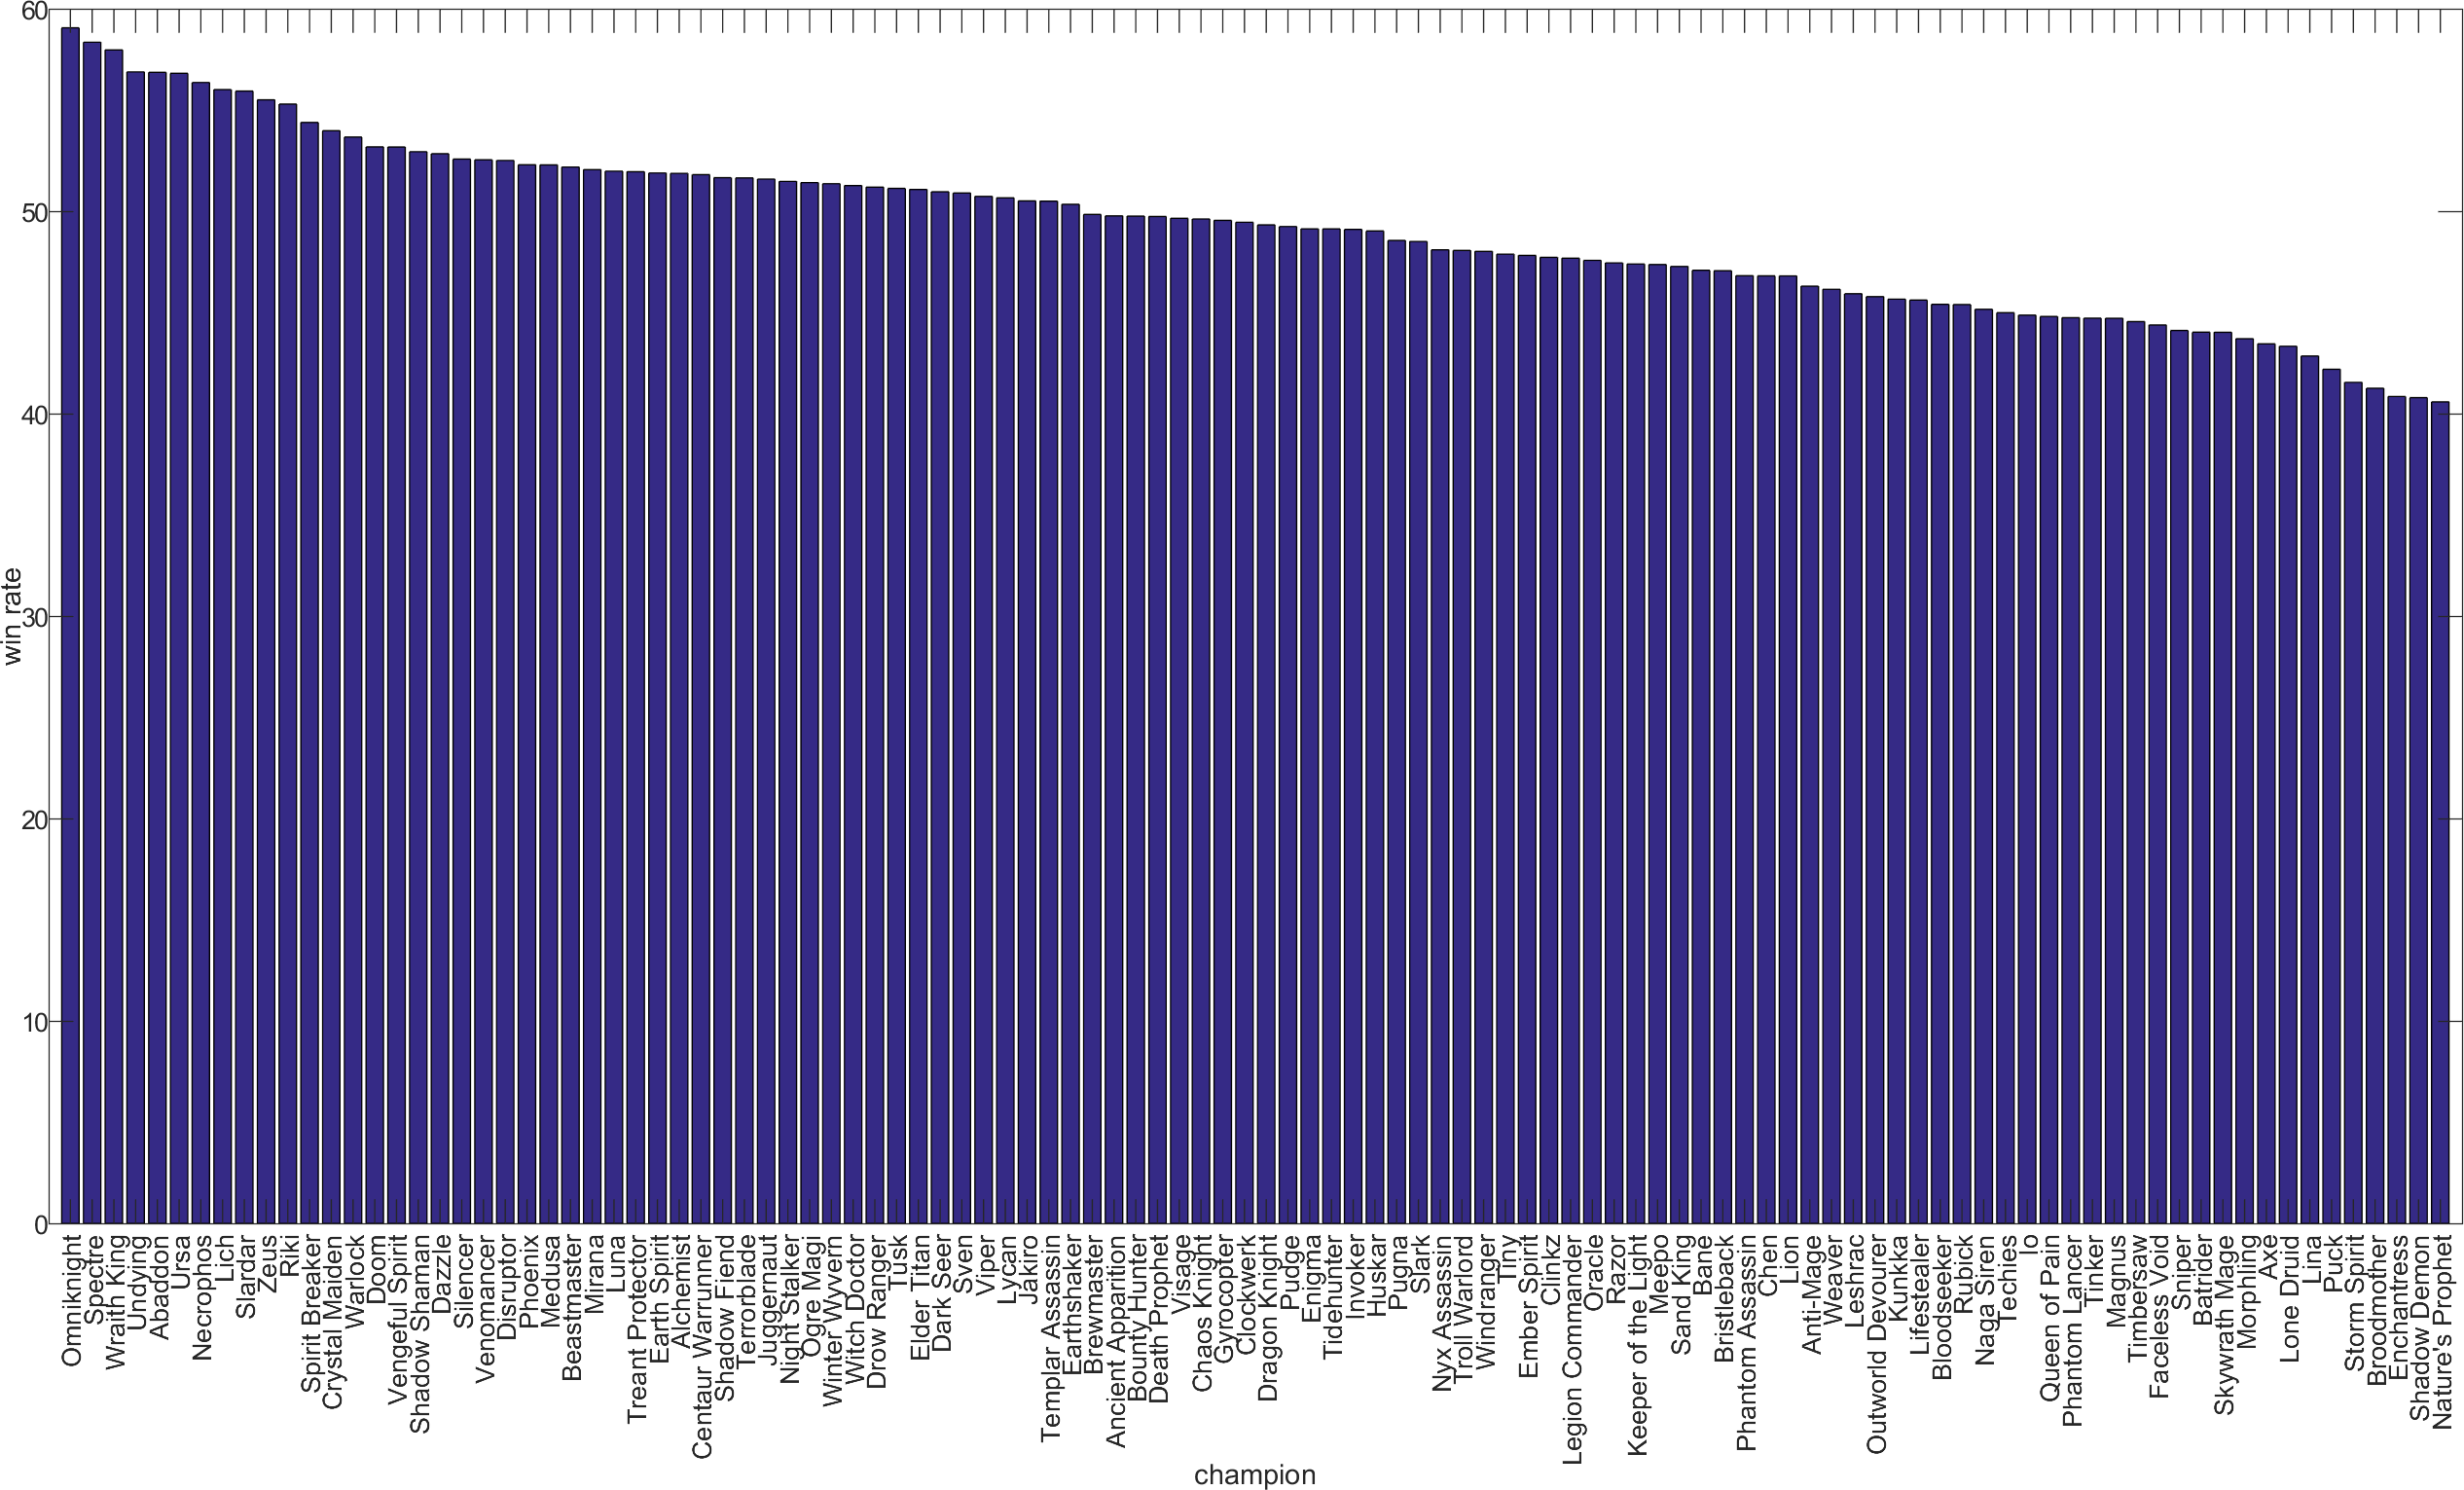
\includegraphics[width=\linewidth]{pics/win_rate.png}
	\caption{Percentuale di vittoria in relazione al campione}
	\label{fig:win_rate}
\end{figure}

\subsection{Percentuale di vittorie in funzione del team}
Successivamente ci siamo chiesti se il team potesse influire sulla percentuale di vittoria. Questa domanda deriva dal fatto che la mappa non è perfettamente simmetrica e questo potrebbe portare un particolare campione ad avere dei vantaggi a giocare in una squadra piuttosto che nell'altra. Le statistiche di vittoria in funzione del team si possono vedere nelle figure \ref{fig:win_by_team_1} e \ref{fig:win_by_team_2}. Come si può vedere dai grafici, per la maggior parte dei campioni non vi è differenza nella vittoria giocando in un team piuttosto che nell'altro. Anche in questo caso, però ci sono alcune eccezioni: per 7 campioni su 110 si ha un significativo vantaggio a giocare una partita nella squadra \textit{Radiant}, mentre per 4 campioni su 110 si ha un vantaggio a giocare nella squadra dei \textit{dire} con la differenza maggiore di circa il 10\% per il campione \textit{Chen}.
\begin{figure}[H]
	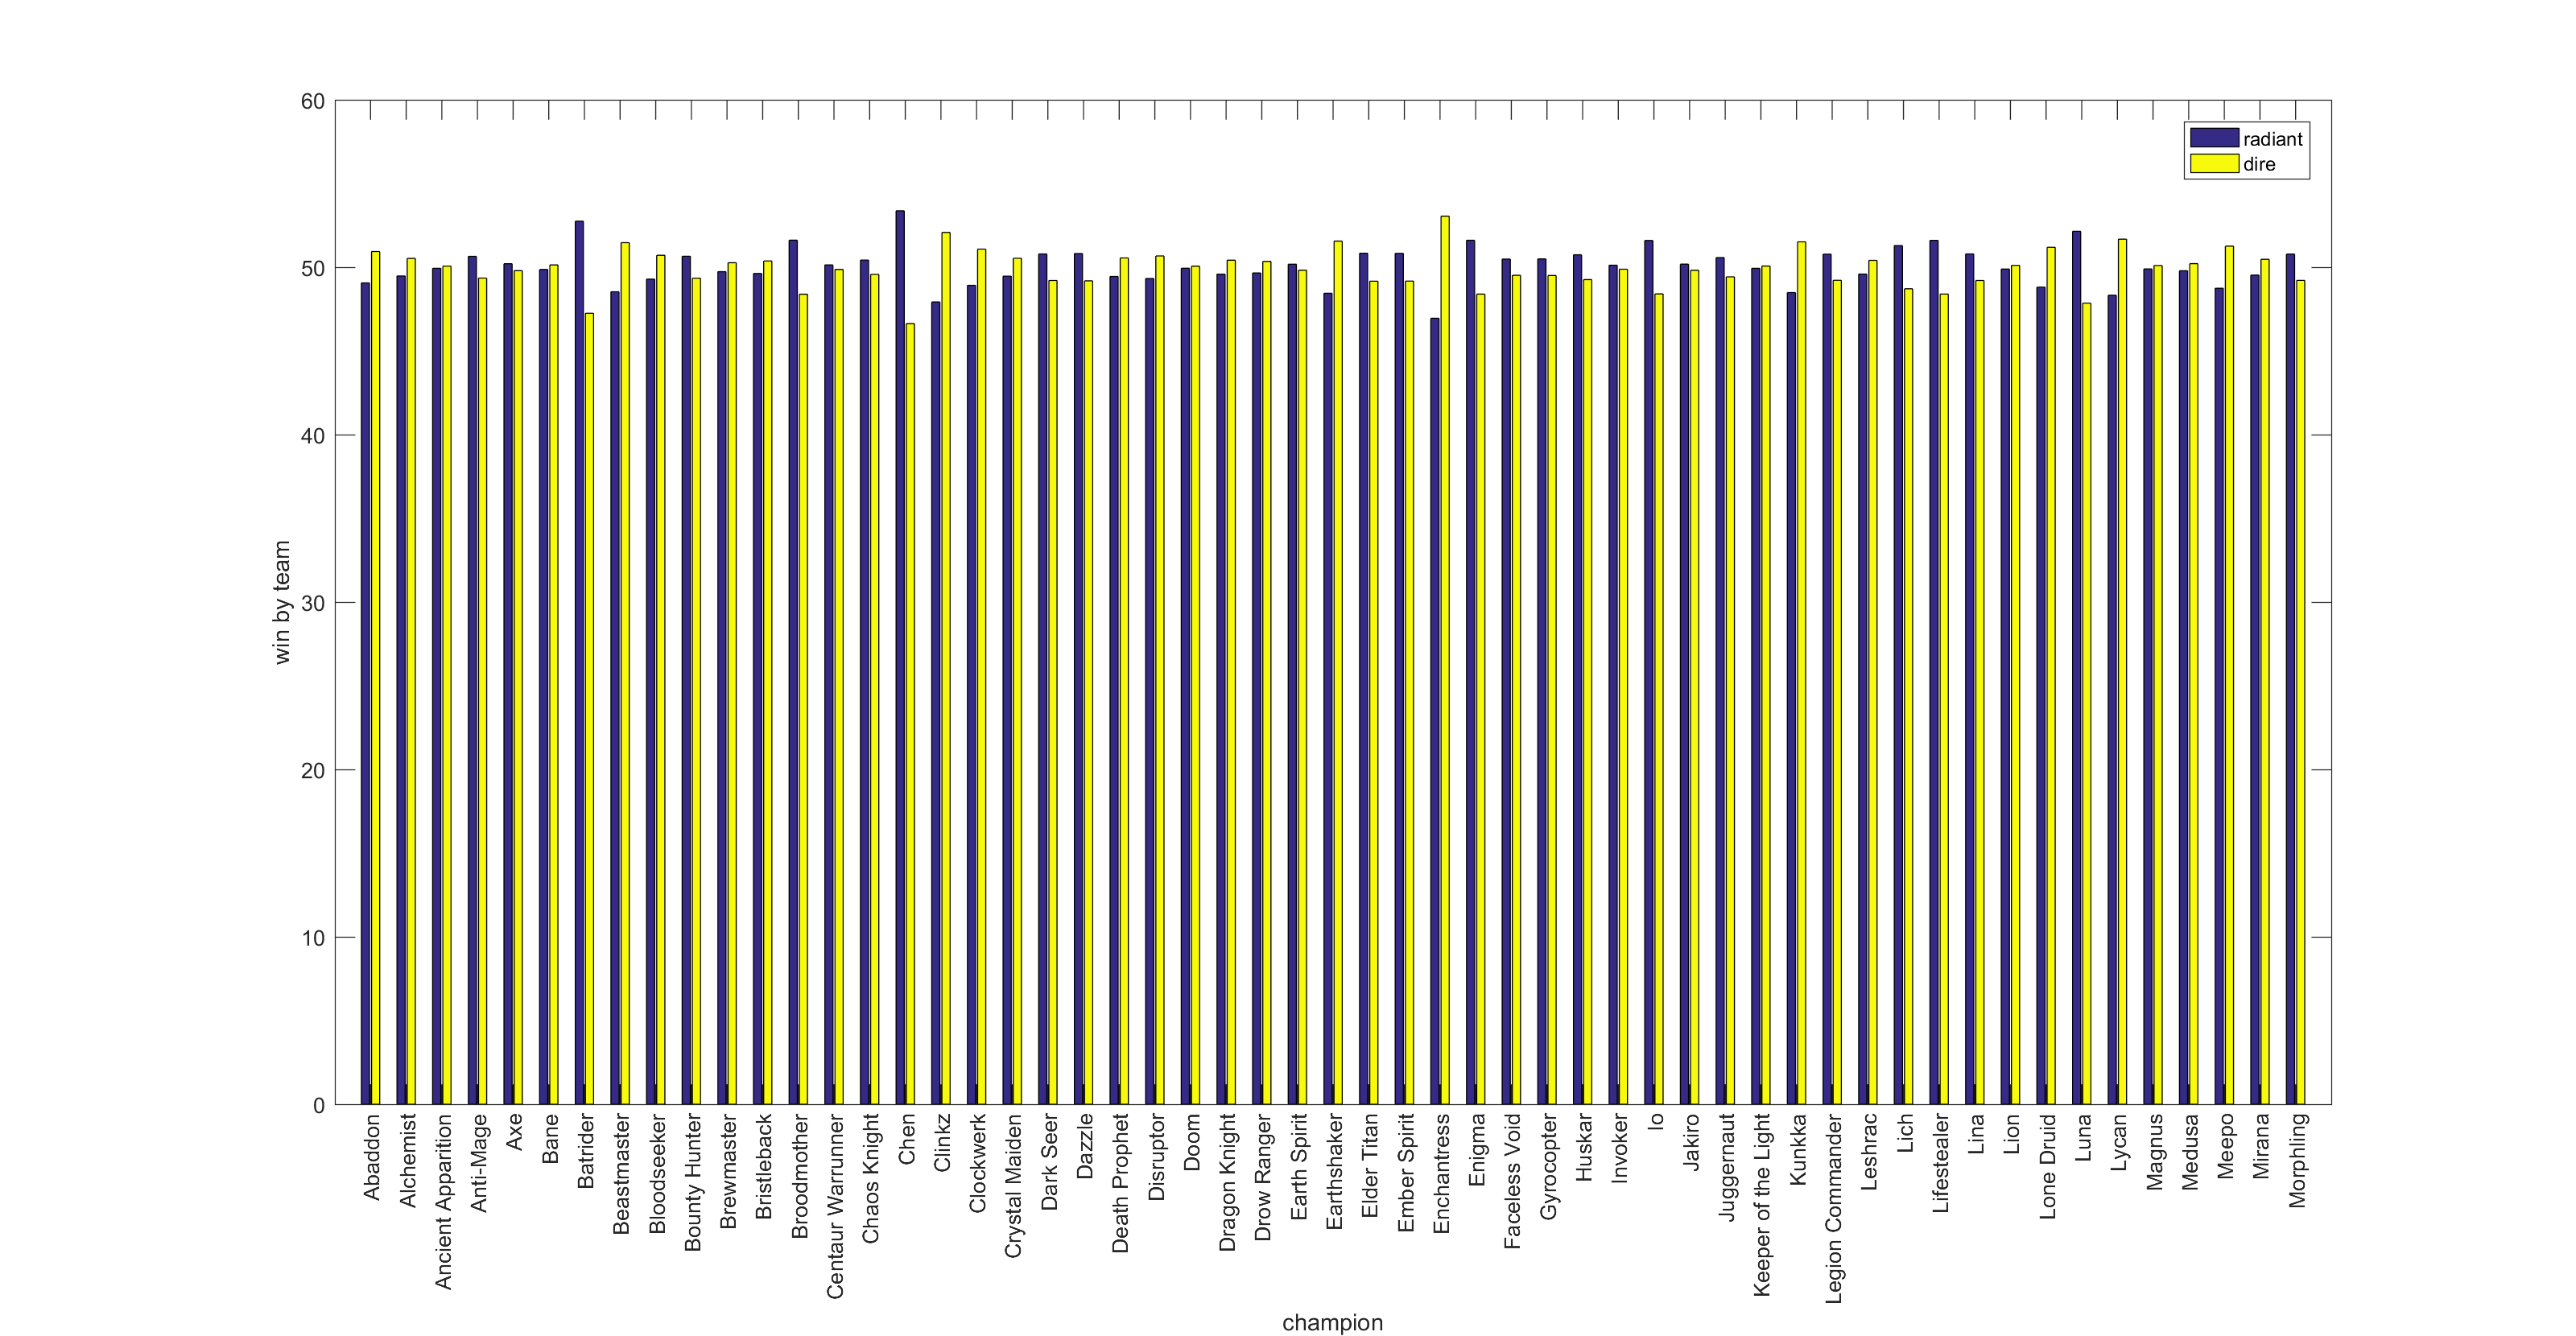
\includegraphics[width=\linewidth]{pics/win_by_team_1.png}
	\caption{Percentuale di vittoria di ogni campione in funzione del team}
	\label{fig:win_by_team_1}
\end{figure}
\begin{figure}[H]
	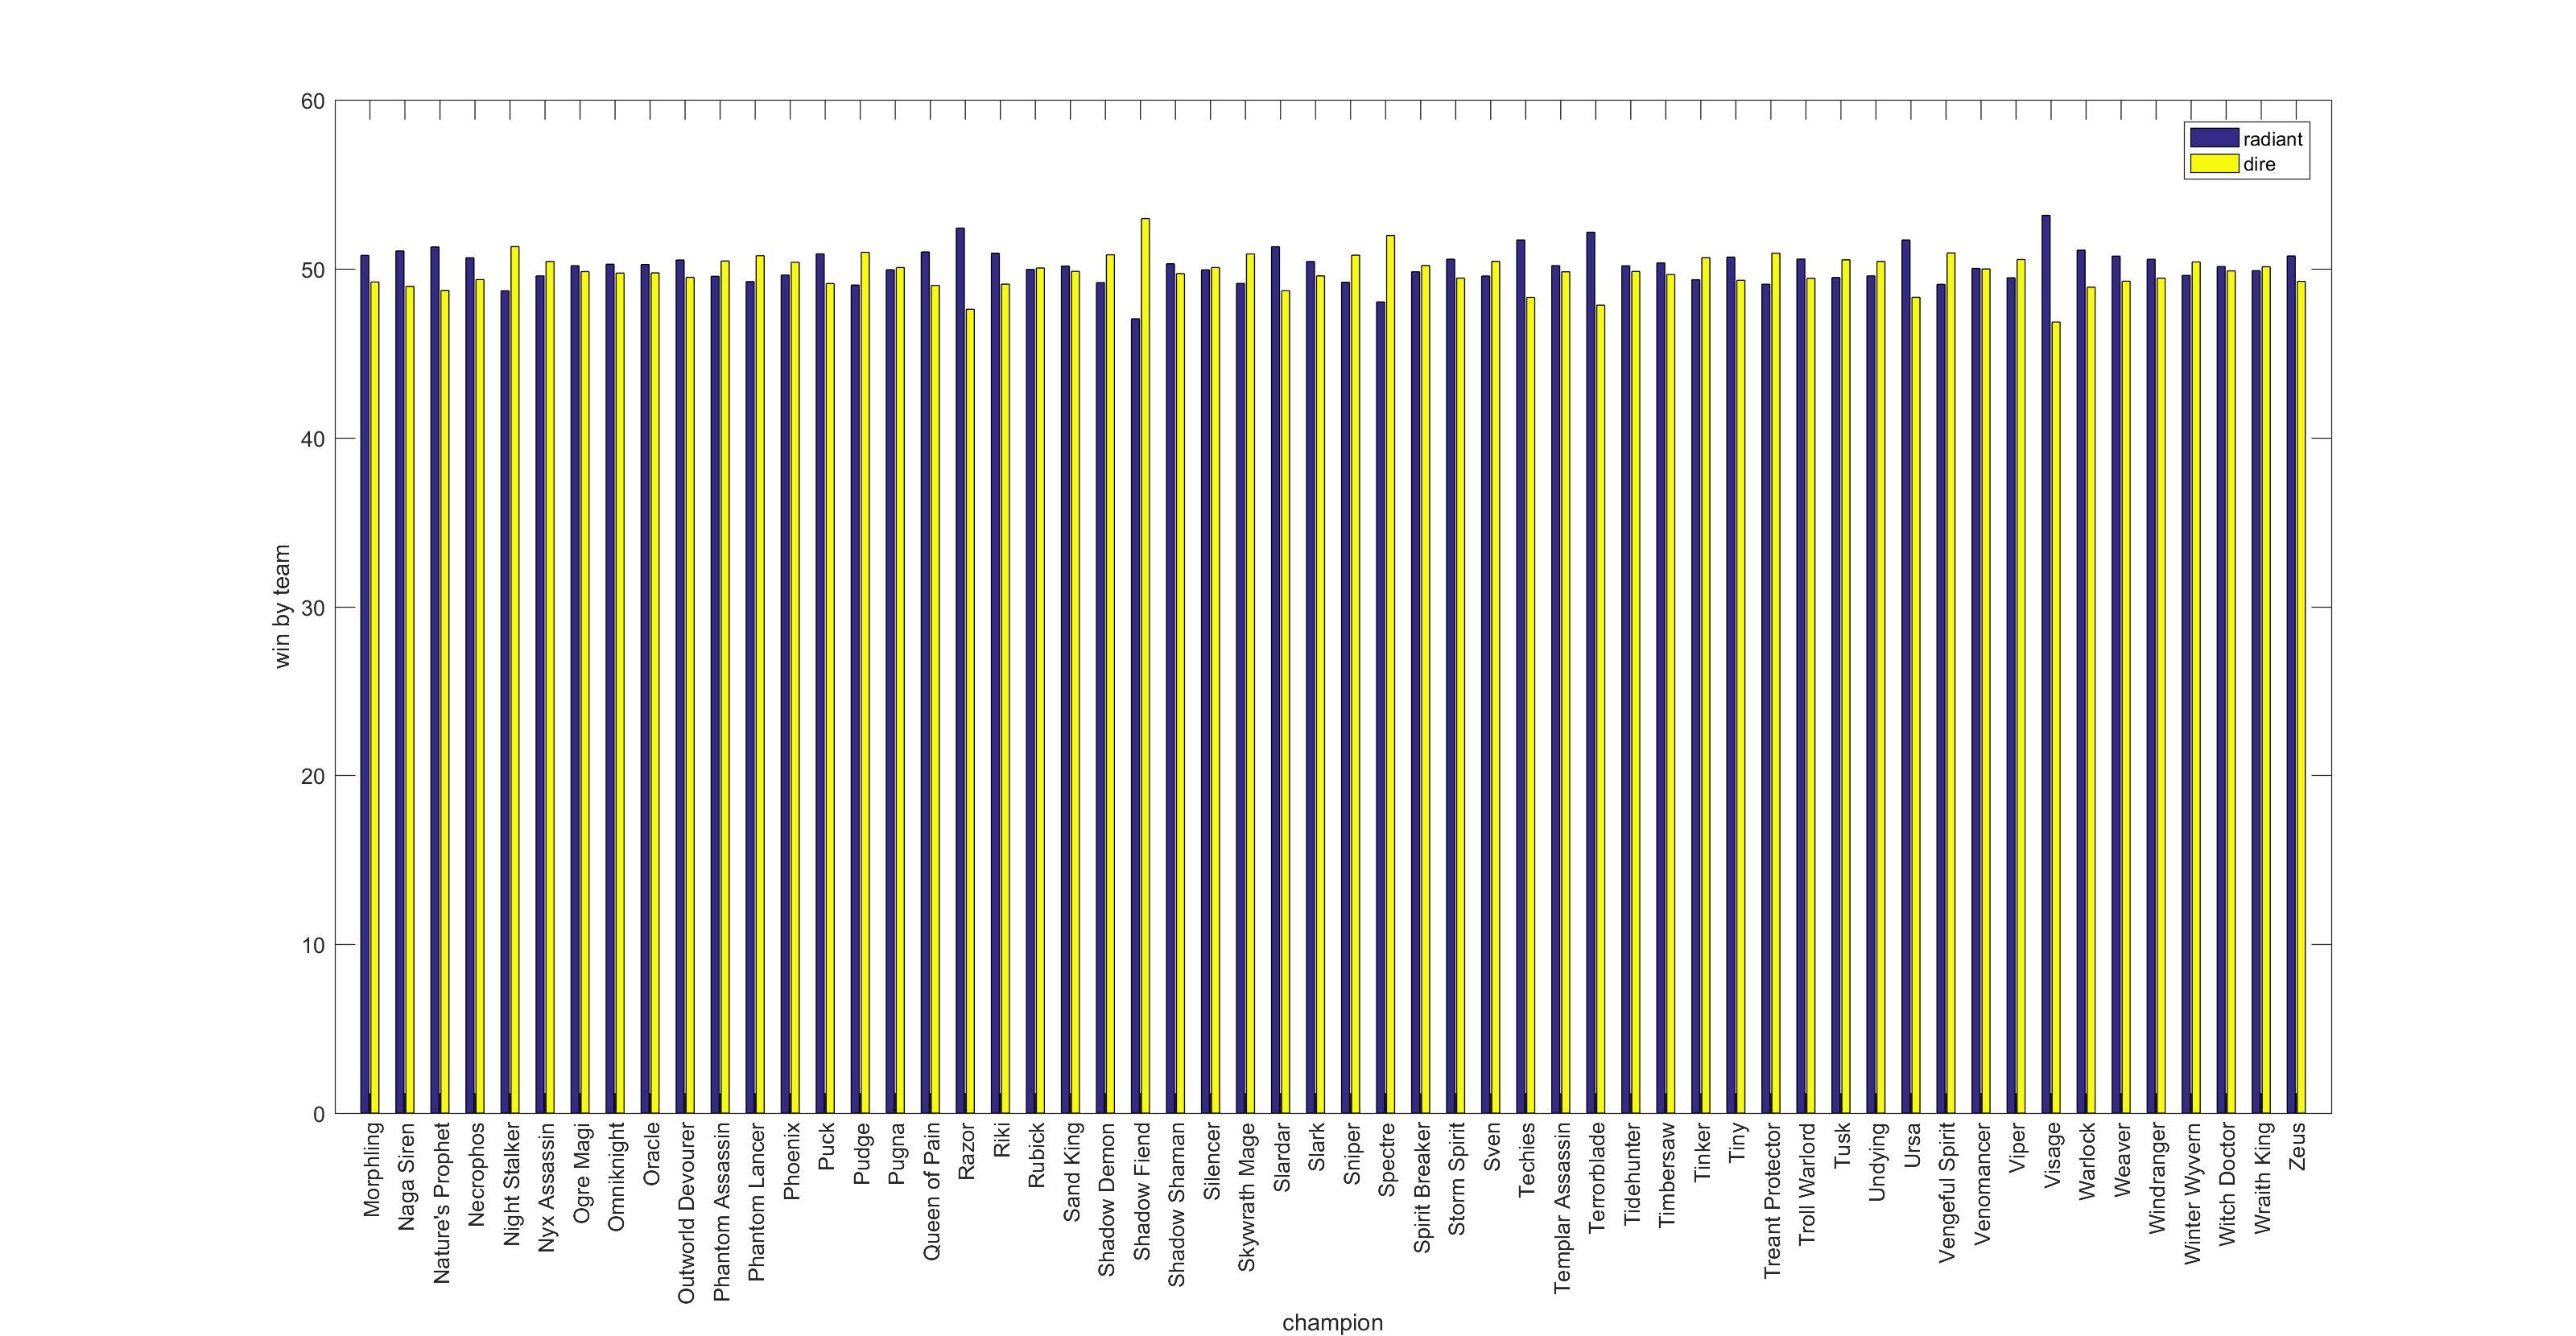
\includegraphics[width=\linewidth]{pics/win_by_team_2.png}
	\caption{Percentuale di vittoria di ogni campione in funzione del team}
	\label{fig:win_by_team_2}
\end{figure}

\subsection{Percentuale di scelta di un campione}
Abbiamo poi calcolato la percentuale di \textit{pick} di un campione, ovvero la probabilità che un campione venga scelto da almeno un giocatore in una partita. Come si può vedere in figura \ref{fig:pick_rate} i campioni \textit{Windranger} e \textit{Shadow Fiend} vengono scelti molto più frequentemente degli altri, ma contrariamente a quanto ci aspettavamo, non sono quelli con una percentuale di vittoria più alta. Si ha poi un secondo gruppo di 25-30 campioni particolarmente popolari e un ultimo gruppo di campioni meno giocati.

\begin{figure}[H]
	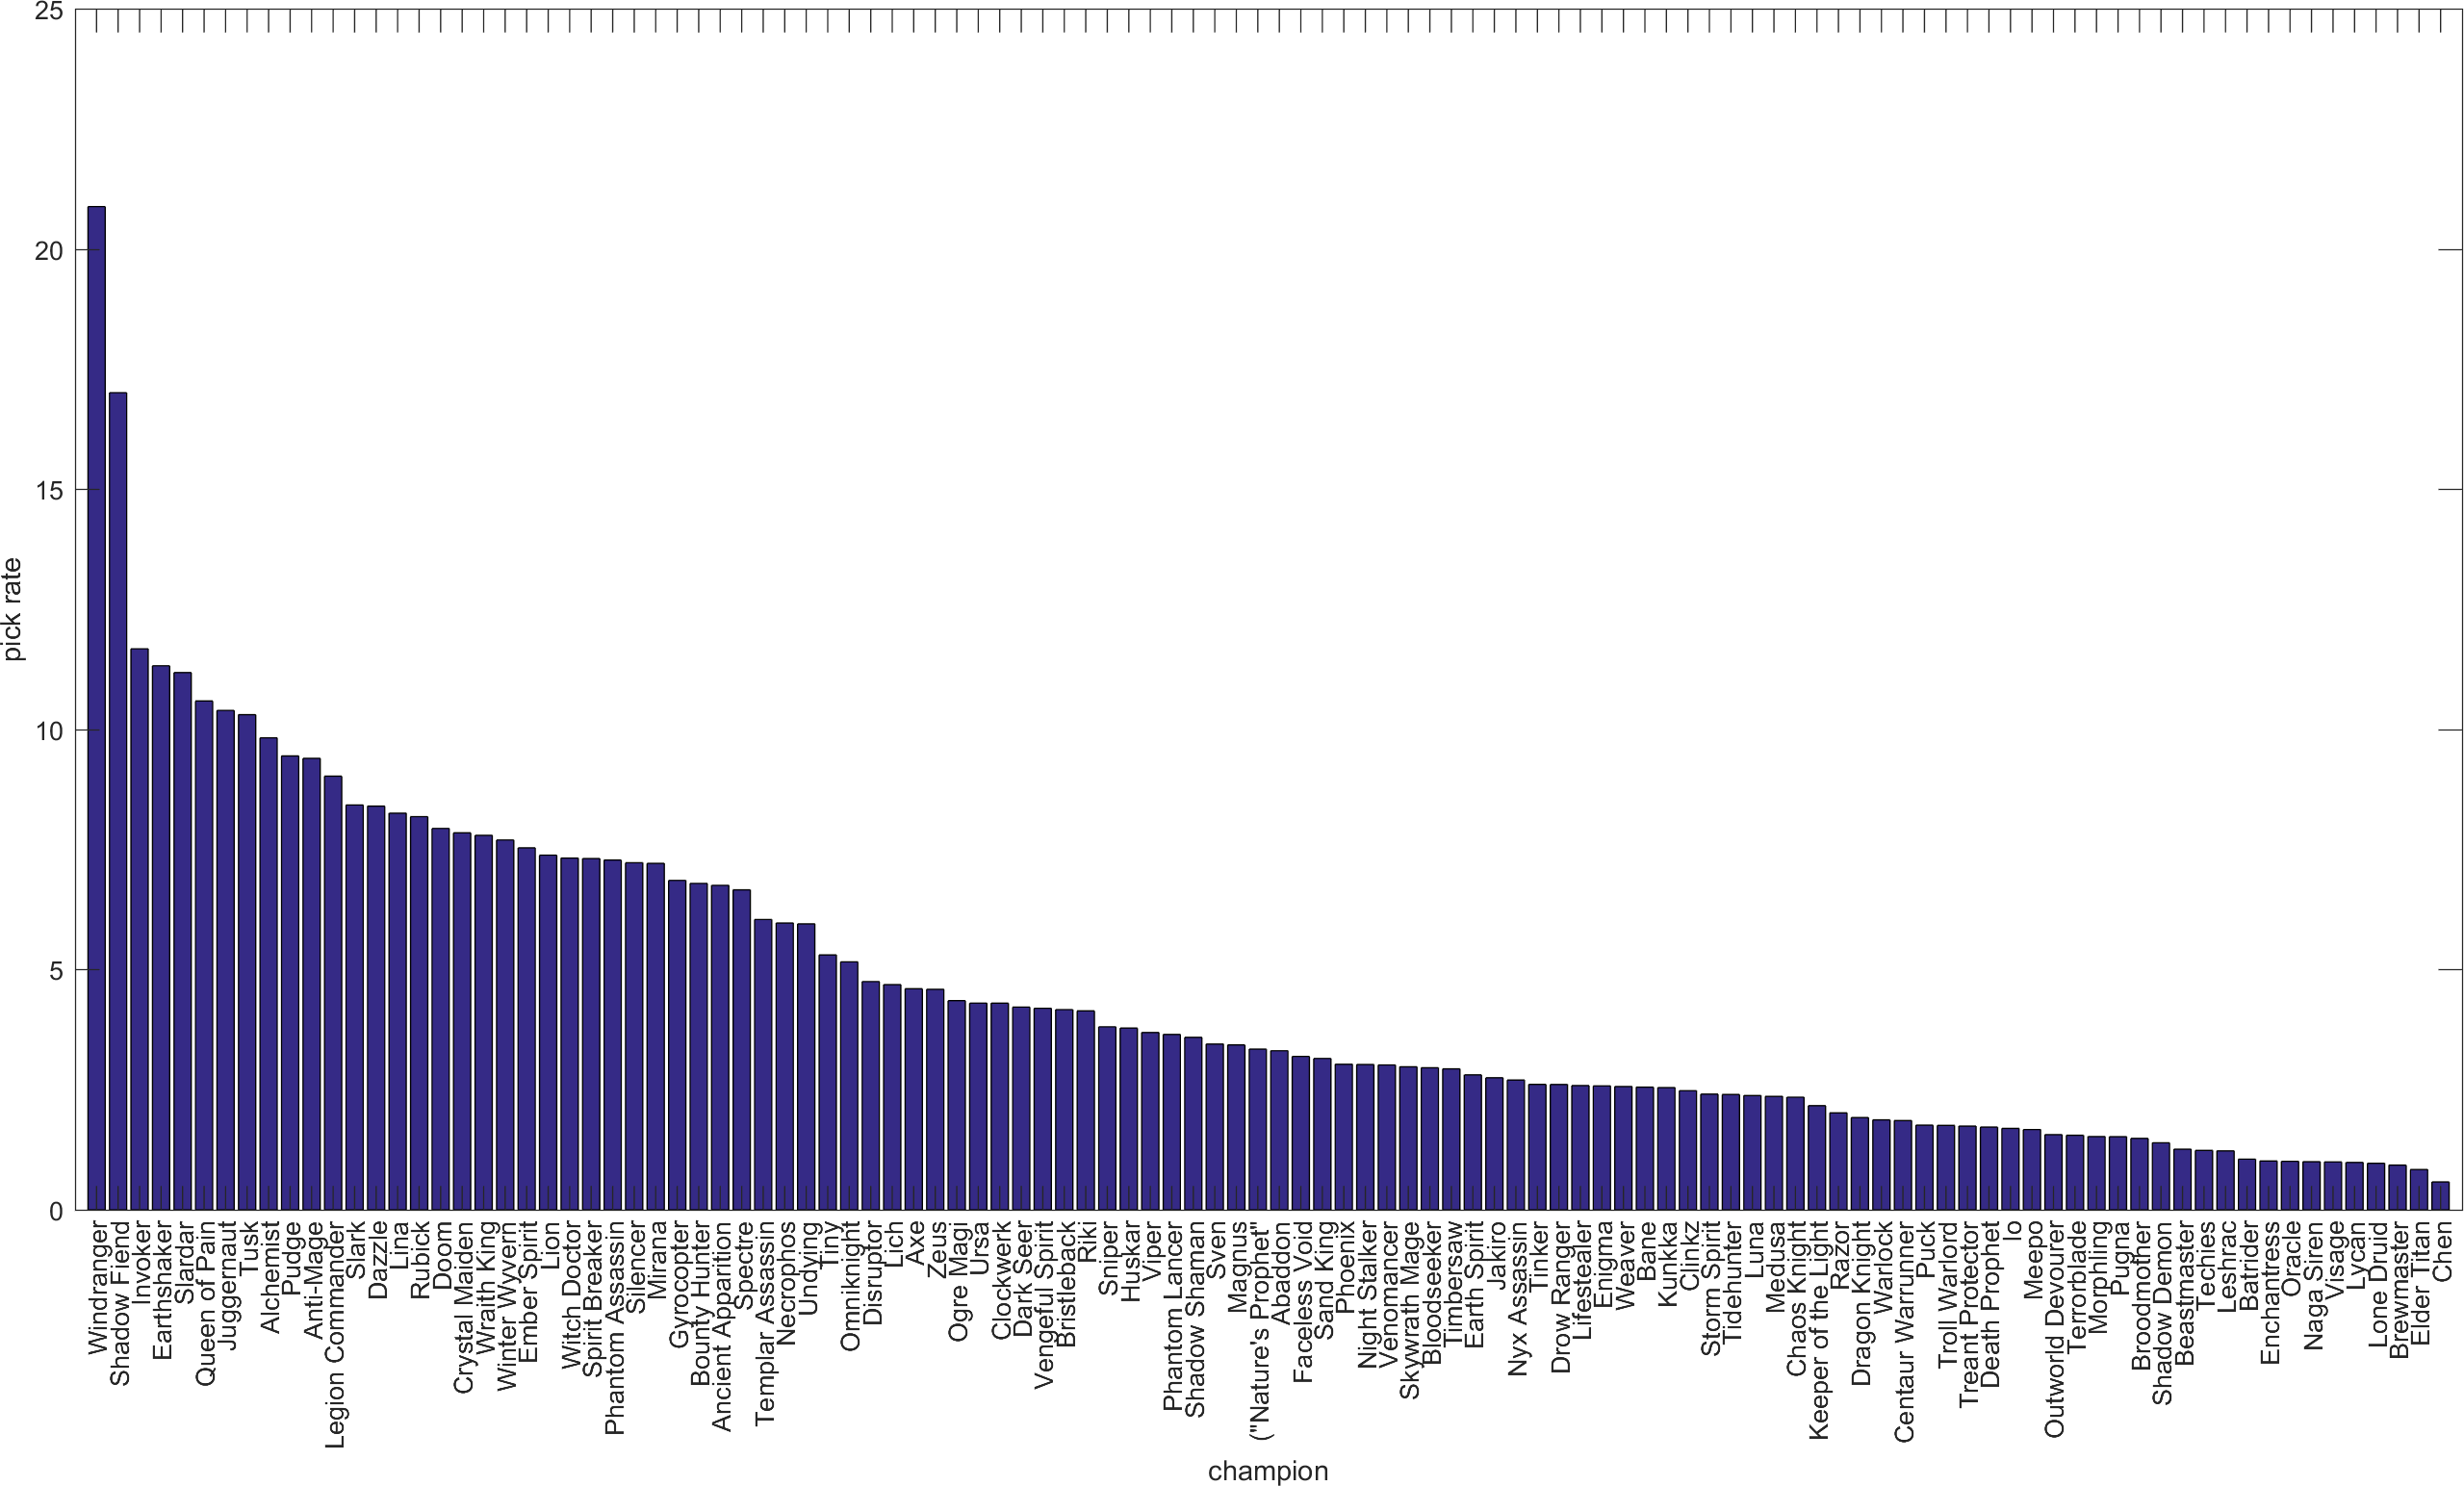
\includegraphics[width=\linewidth]{pics/pick_rate.png}
	\caption{Percentuale di scelta di un campione}
	\label{fig:pick_rate}
\end{figure}

\subsection{Durata media delle partite}
Un'altra statistica calcolata è la durata media di una partita calcolata utilizzando il dataset \verb|matches_stats| e riportata in figura \ref{fig:average_duration} e risulta essere di circa quaranta minuti.
\\
In figura \ref{fig:duration_by_champ} è riportata invece la durata media di una partita per ogni campione. Come ci aspettavamo, la scelta del campione non influisce nella durata, ma anche in questo caso di sono due accezioni anche se la differenza è comunque ridotta.


\begin{figure}
	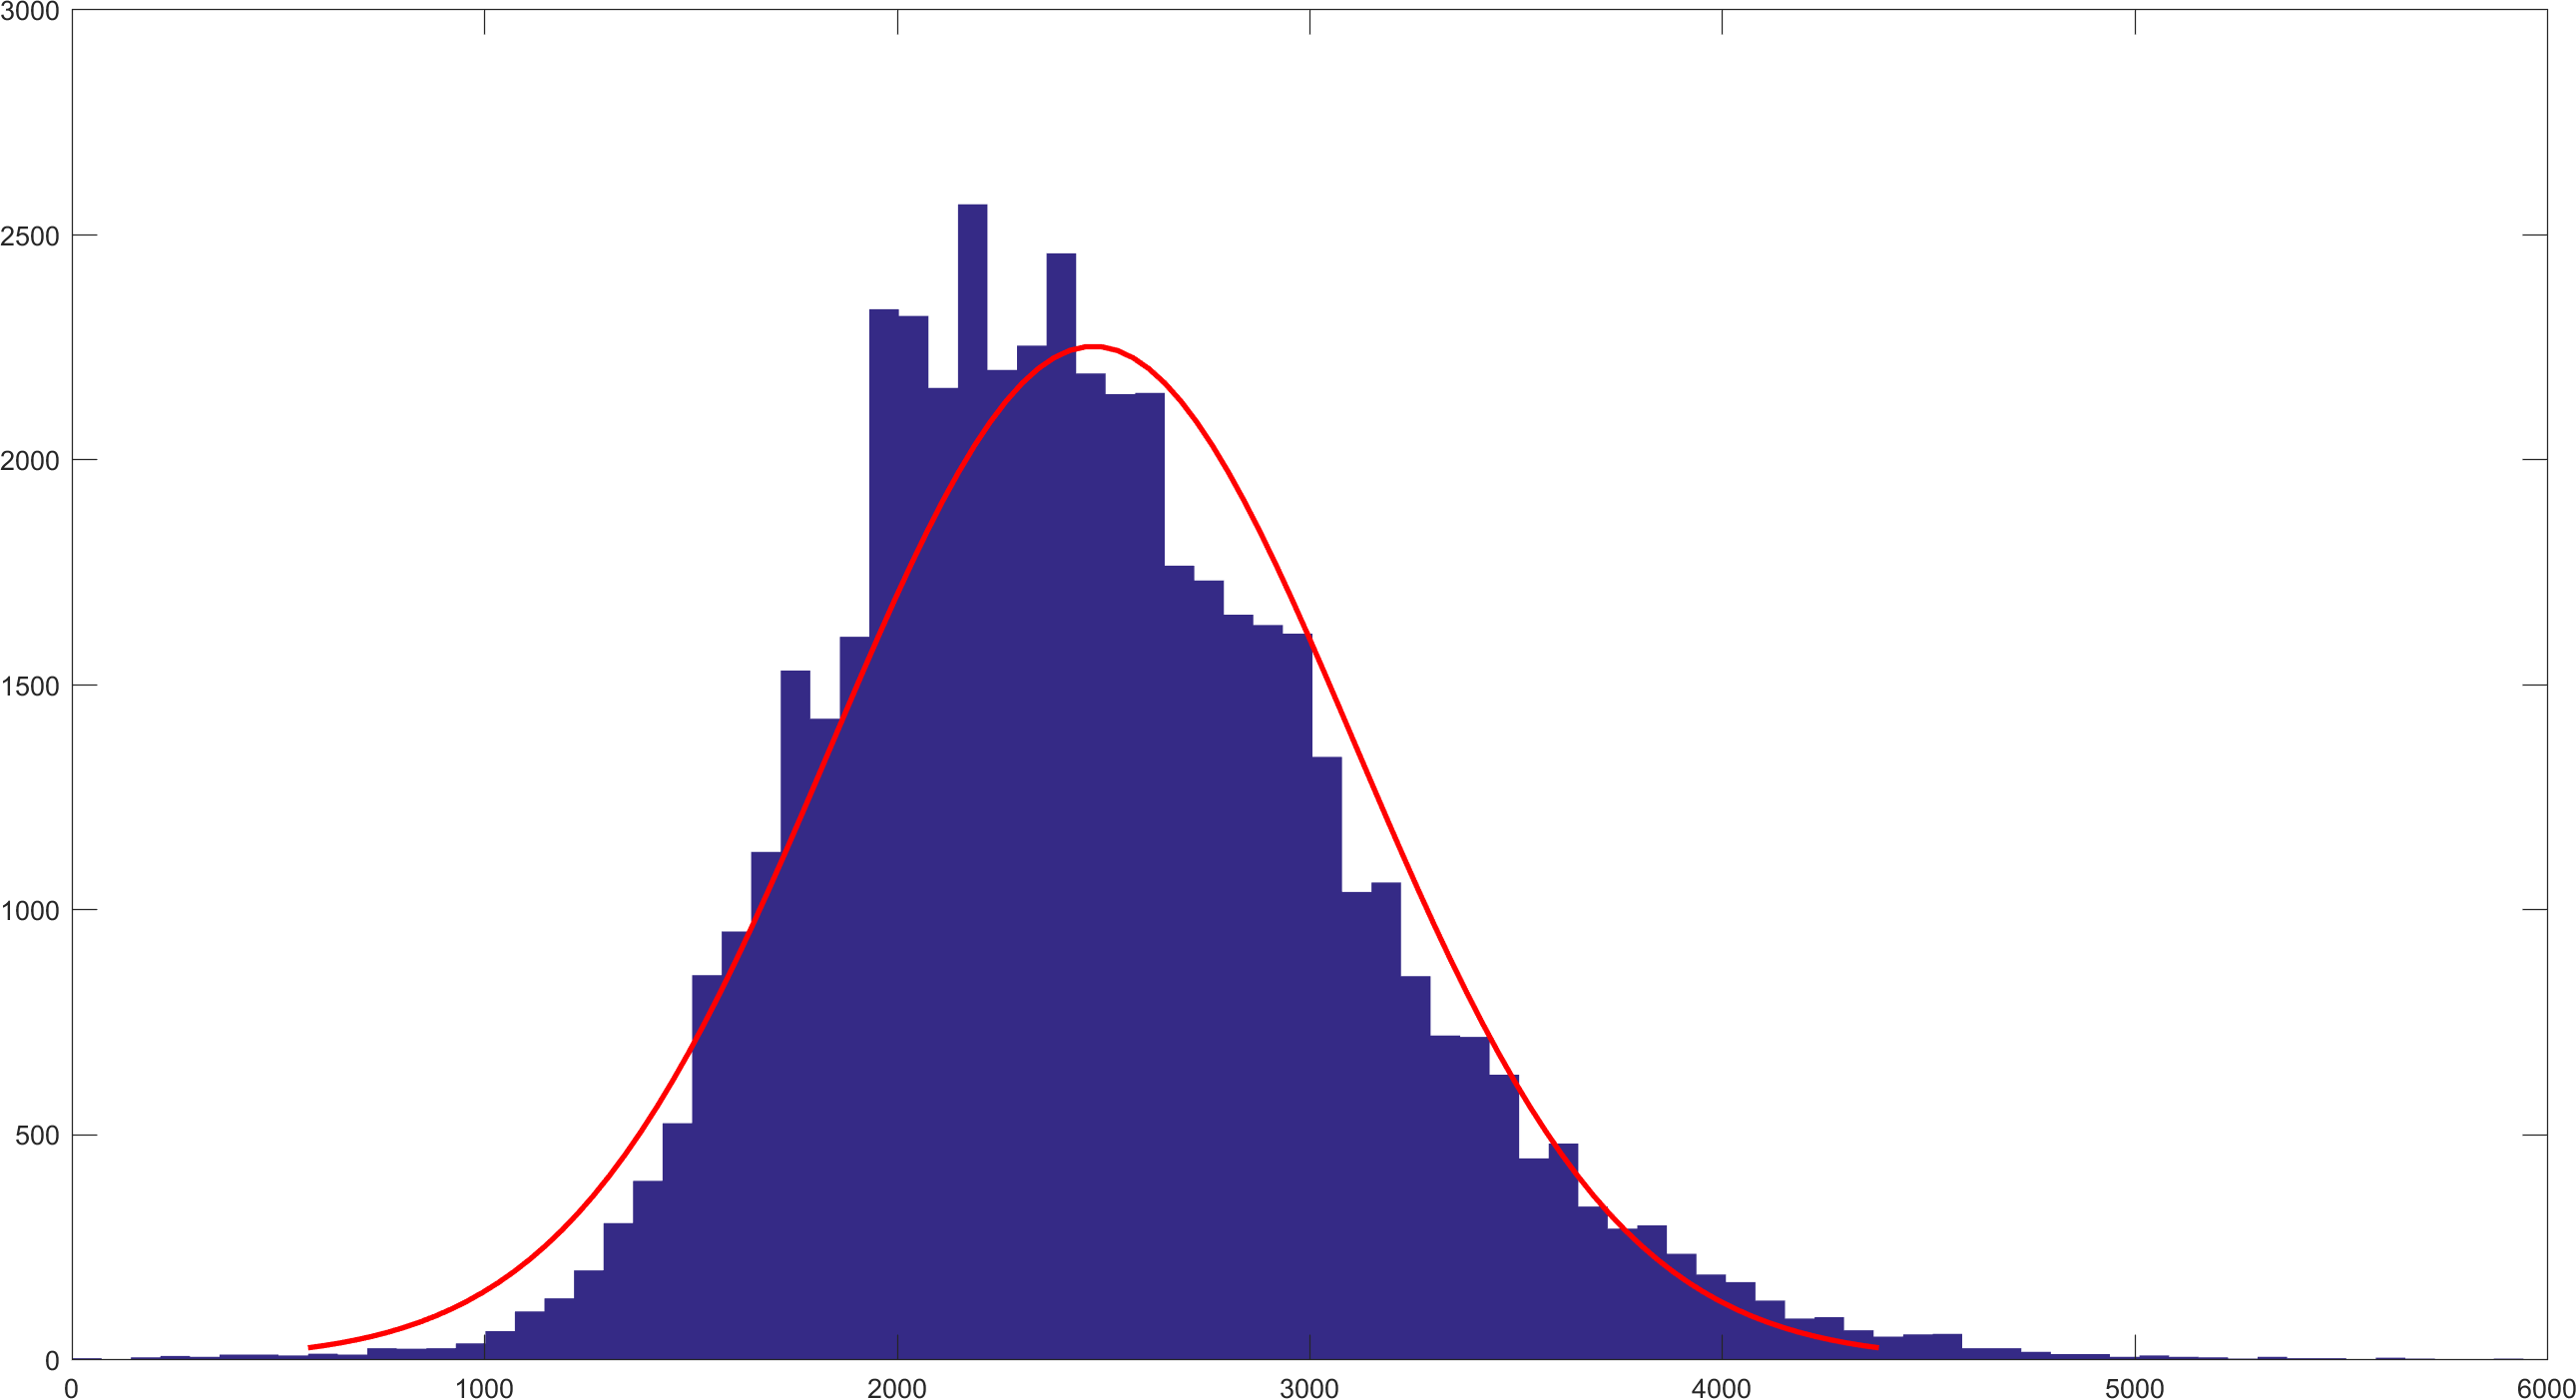
\includegraphics[width=\linewidth]{pics/average_duration.png}
	\caption{Durata media di una partita}
	\label{fig:average_duration}
\end{figure}

\begin{figure}
	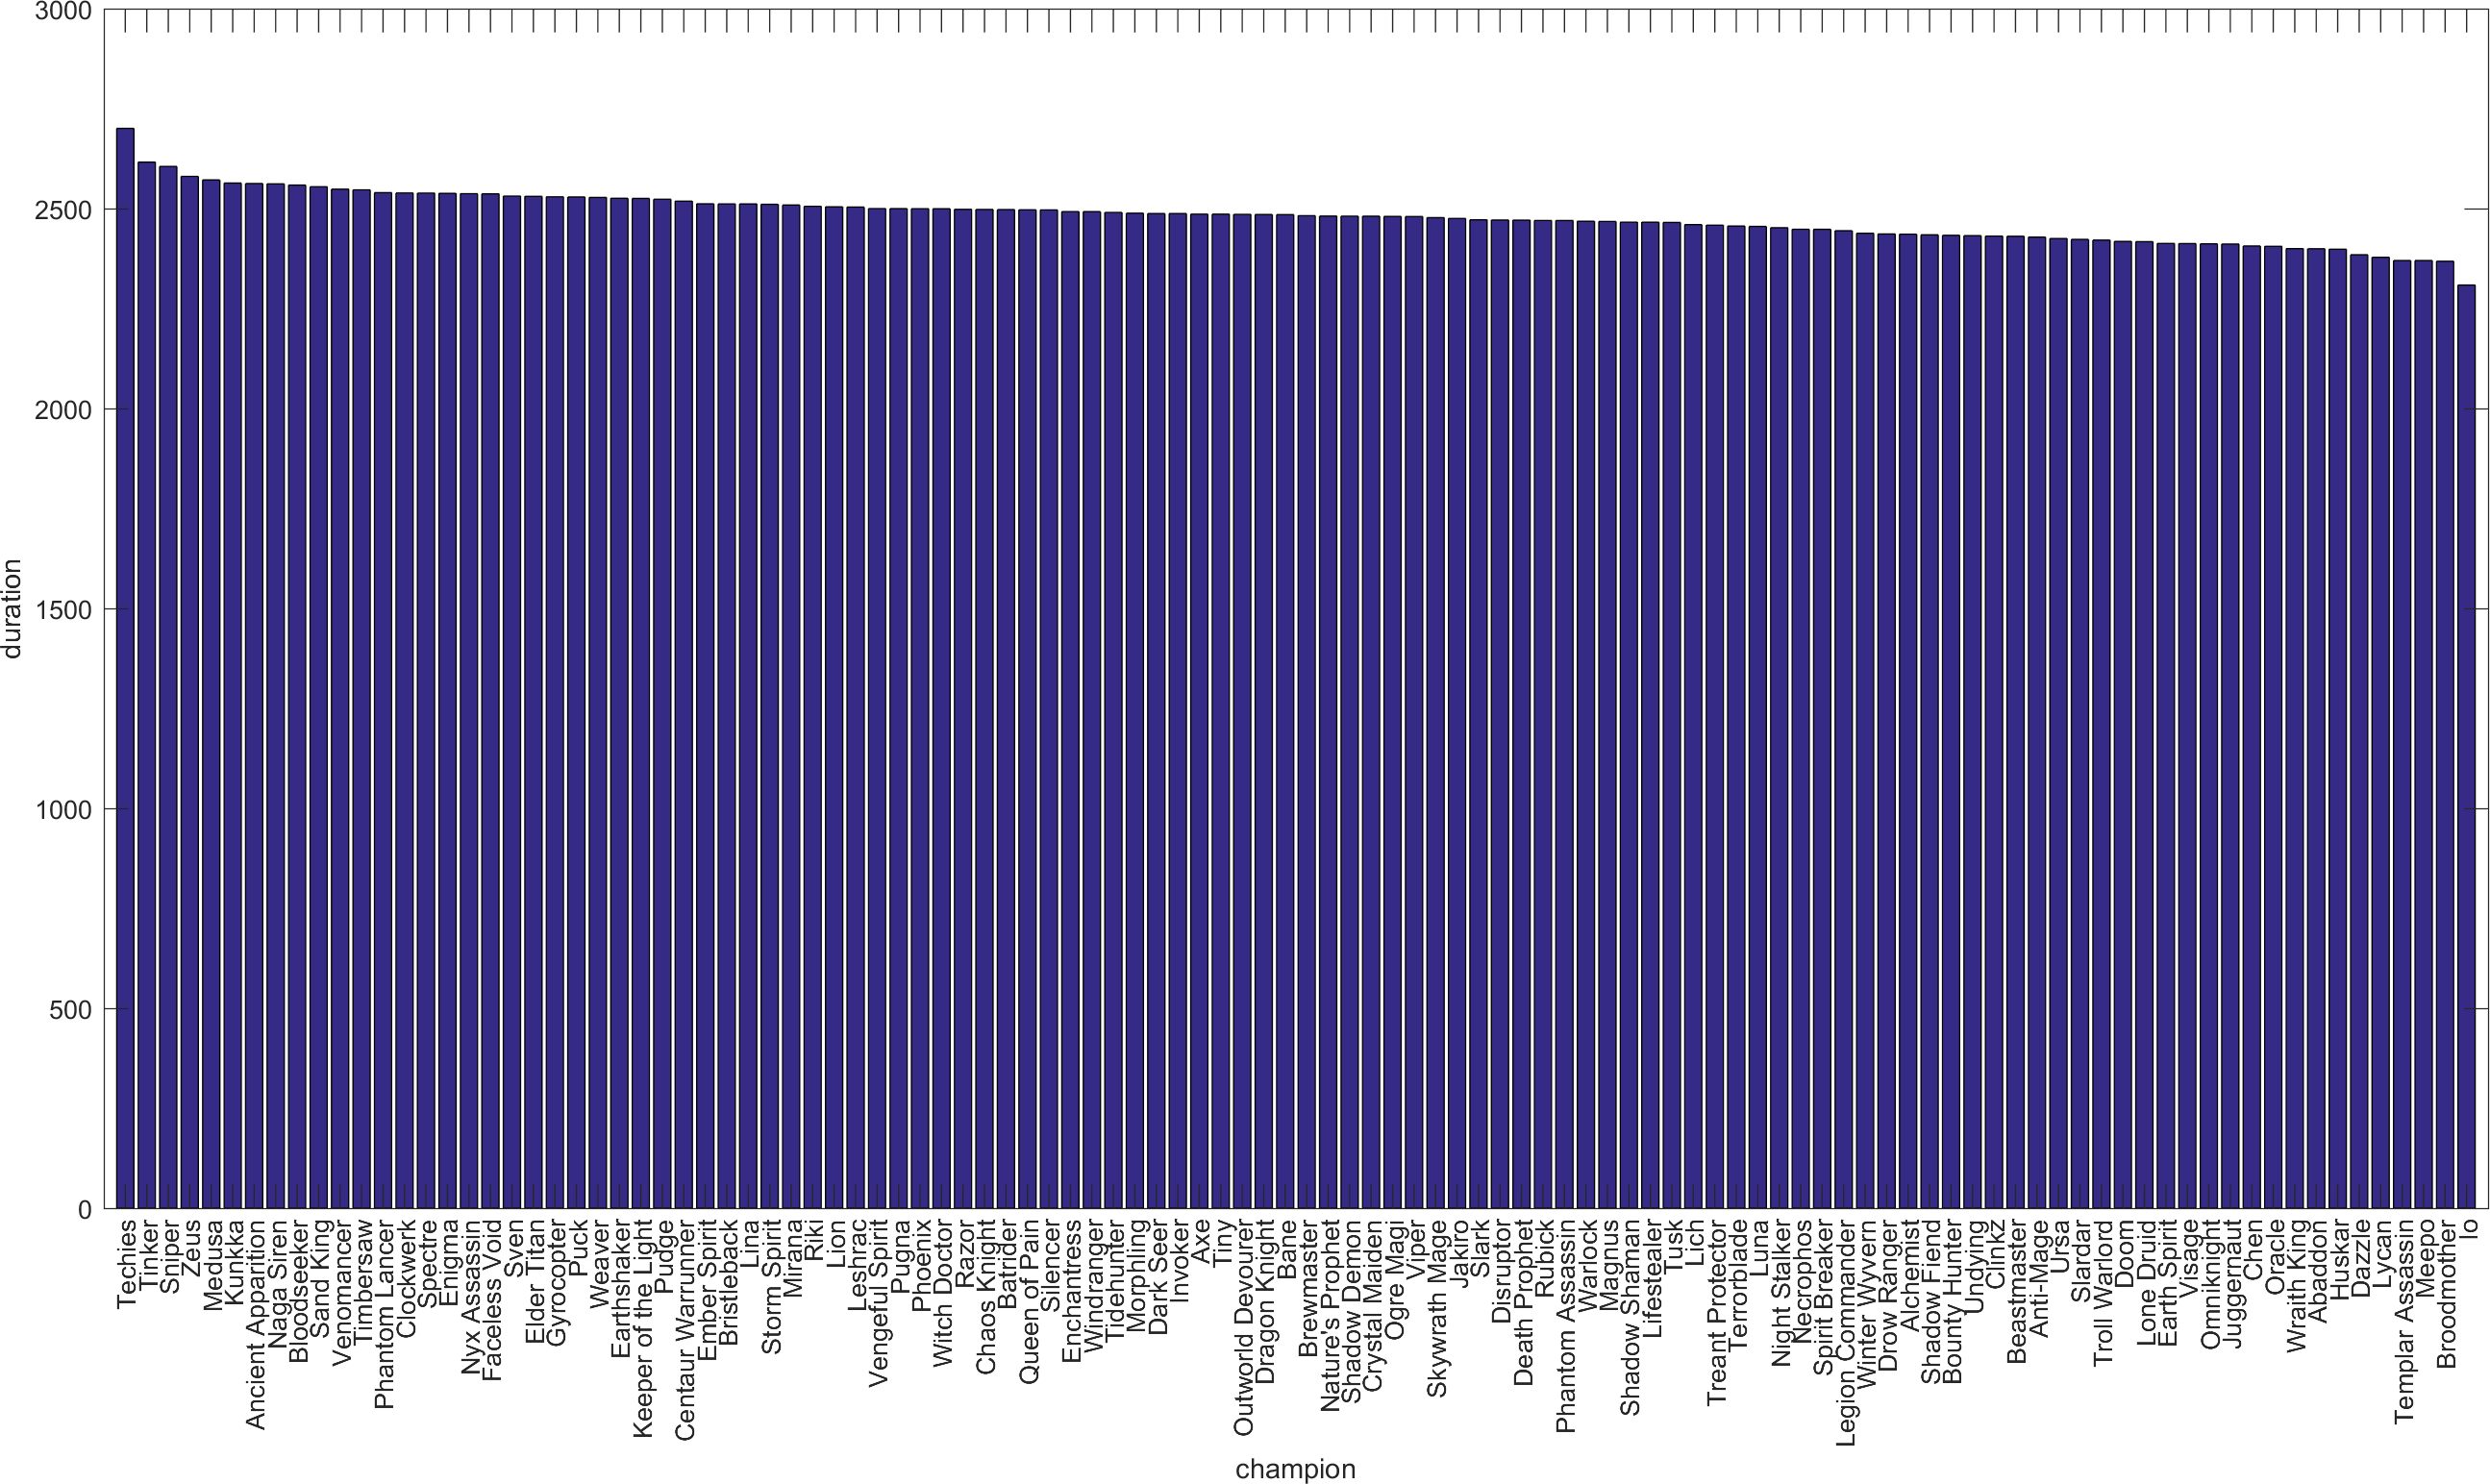
\includegraphics[width=\linewidth]{pics/duration_by_champ.png}
	\caption{Durata media di una partita in funzione del campione scelto}
	\label{fig:duration_by_champ}
\end{figure}

\subsection{Percentuale di vittoria in funzione della durata di una partita}
Abbiamo poi provato a calcolare quale fosse la percentuale di vittoria di ogni campione in funzione della durata di una partita in modo da evidenziare \textit{champion} che tendono a performare meglio durante il \textit{late game} (la fase finale del gioco) e durante l'\textit{early/mid game} (le fasi iniziali e intermedie). Le partite sono state suddivise in bucket di cinque minuti ciascuna dopo aver eliminato una partita outlier della durata di 16 000 secondi. Abbiamo poi calcolato la percentuale di vittoria di ogni campione per ognuno dei bucket calcolati e trovato una curva che meglio approssimasse i valori trovati. Per quest'ultima parte abbiamo utilizzato la libreria \verb|numpy| ed effettuato il fit con un polinomio di terzo grado. Il metodo di ricerca degli outlier non è estremamente affidabile e, come si può vedere in figura \ref{fig:win_by_length}, per alcuni campioni la curva trovata non rispecchia correttamente le percentuali (in particolare si può osservare quella del campione \textit{Spirit Breaker}). Per questo motivo sono stati plottati anche i punti utilizzati per effettuare la regressione.
\begin{figure}[H]
	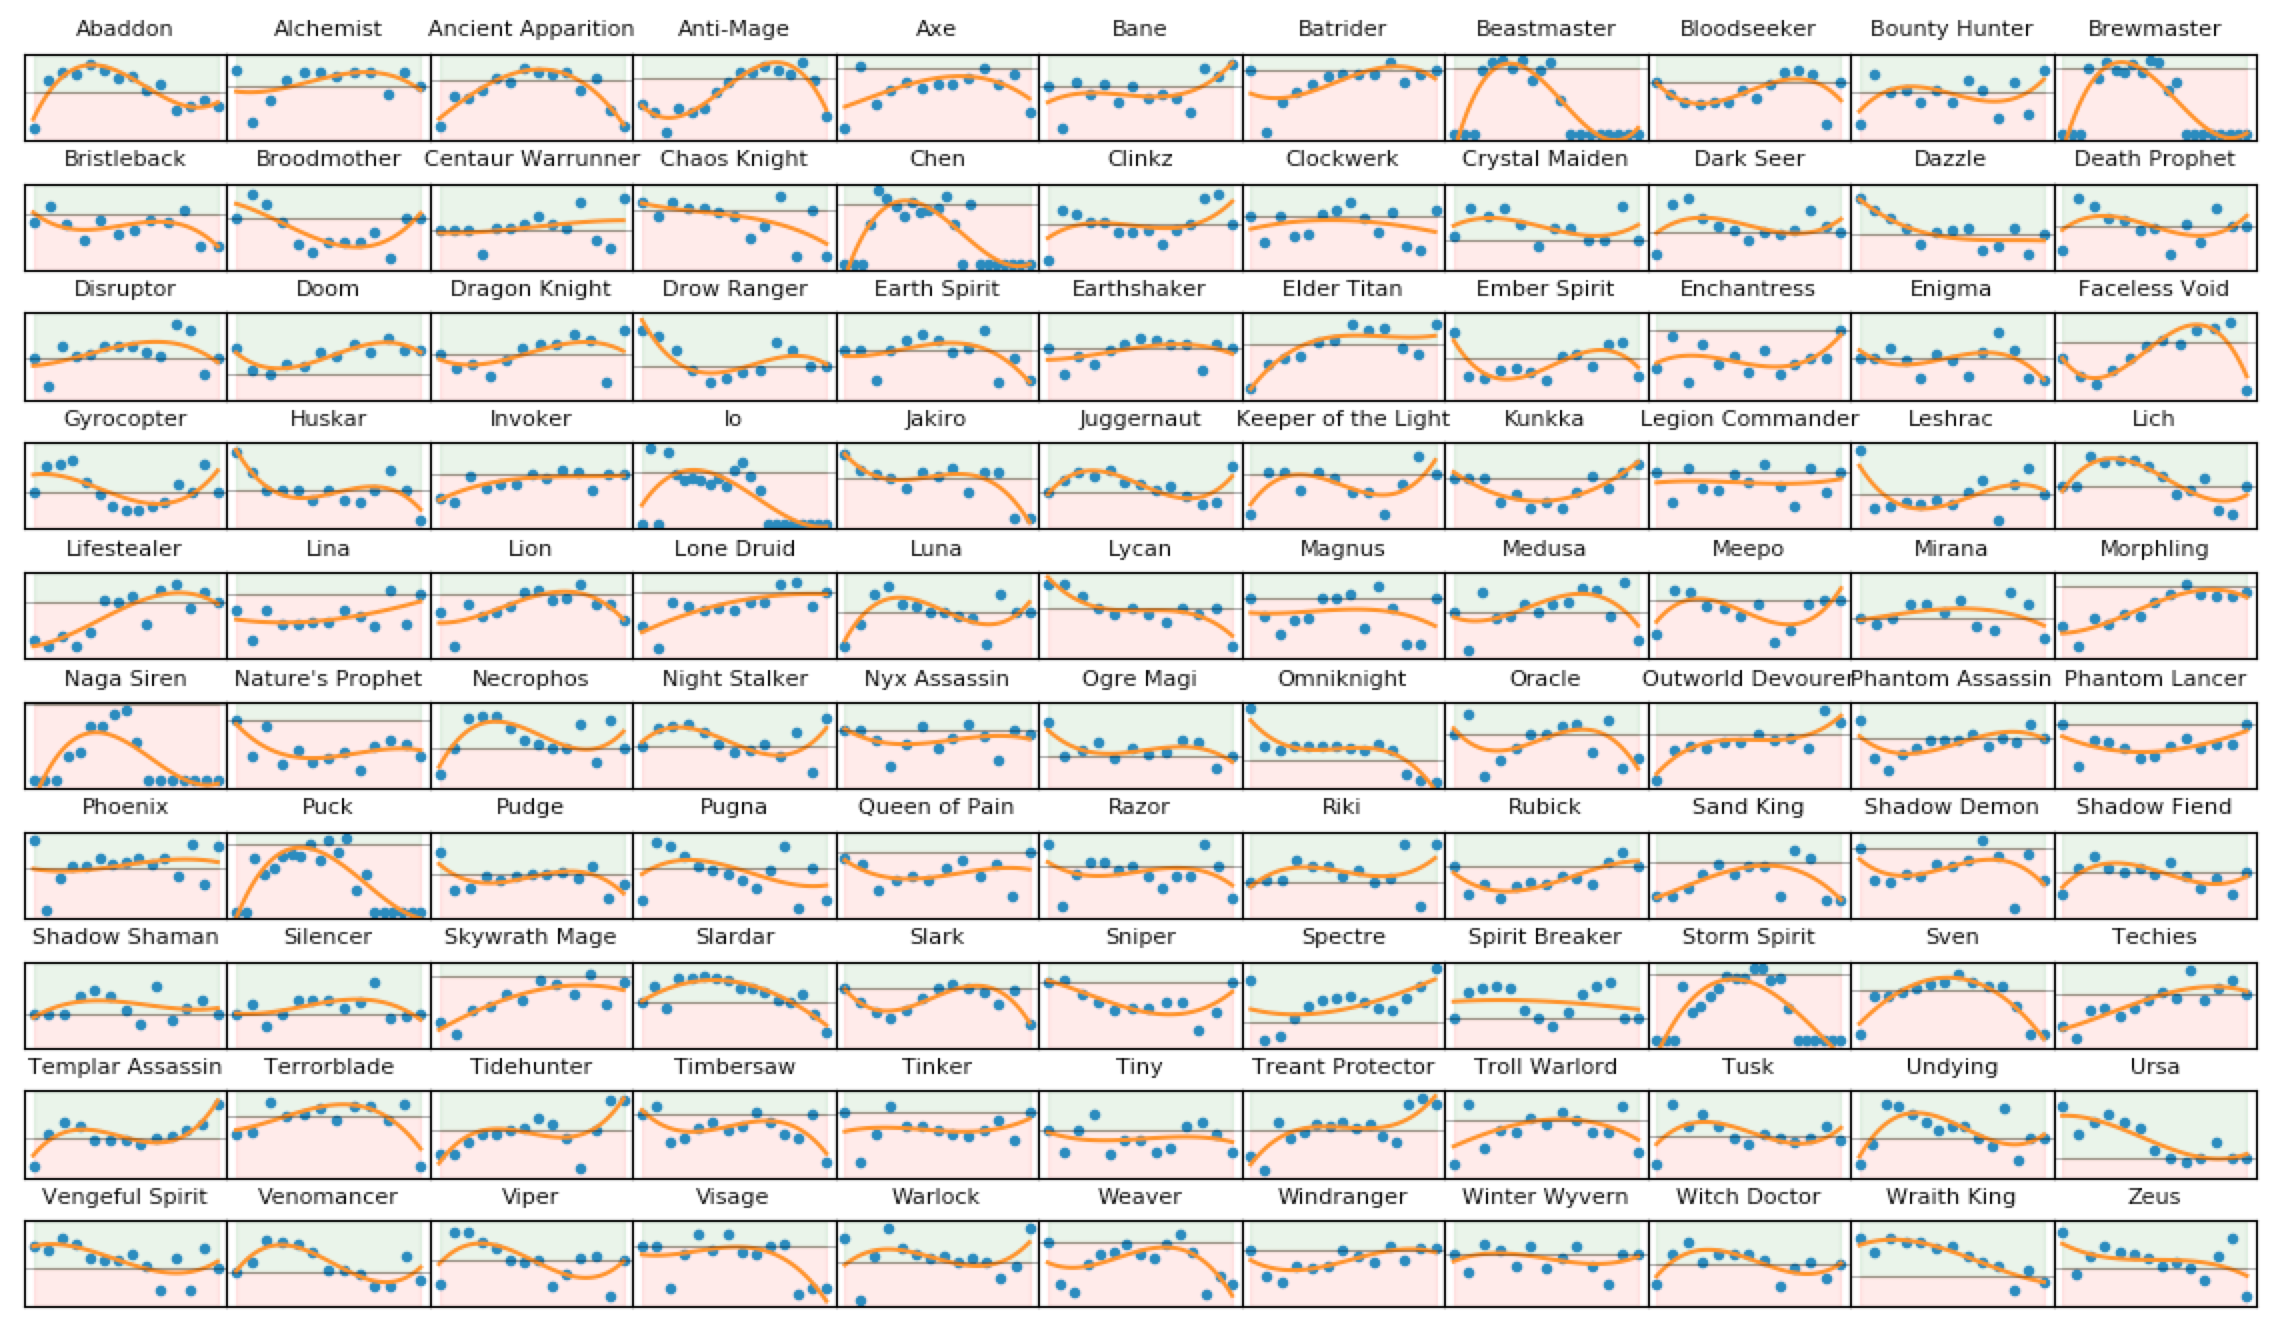
\includegraphics[width=\linewidth]{pics/win_by_len.png}
	\caption{Percentuale di vittoria di ogni campione in funzione della durata della partita}
	\label{fig:win_by_length}
\end{figure}




\chapter{Machine Learning}


\section{Descrizione del problema}
L'obiettivo di questo progetto è quello di cercare, tramite algoritmi di clusterizzazione, in che modo sono strutturati i dati da analizzare. Per completare questo task è stato utilizzato l'algoritmo di unsupervised-learning k-means. Il dataset che è stato utilizzato contiene tutte le caratteristiche dei personaggi del videogioco DOTA2. Di conseguenza, applicare un algoritmo di unsupervised-learning su un dataset di questa tipologia equivale a suddividere in categorie di "forza" i vari champions.\\
Essendo la natura del gioco quella di rendere il gameplay il più equilibrato possibile, individuare delle categorie di personaggi non è una pratica facile come può sembrare, anche perché la "forza" di un personaggio è stimata osservando diverse caratteristiche.
\section{Analisi del dataset}
Il dataset utilizzato per il clustering è composto da 13 features di cui una non è stata utilizzata in quanto contiene il nome del personaggio. Le altre 12 features rappresentano:
\begin{itemize}
	\item hero\_name : il nome del campione;
	\item kills : numero medio di uccisioni del \textit{champion};
	\item deaths : numero medio di morti del \textit{champion};
	\item assists : numero medio di partecipazioni alle uccisioni; 
	\item lasthits : numero medio di \textit{creep} uccisi;
	\item hero\_damage : danno medio inflitto dal giocatore;
	\item hero\_healing : danni medio curati dal giocatore;
	\item tower\_damage : danni medi inflitti alle torri;
	\item gold\_over\_duration : monete medie guadagnate al secondo;
	\item xp\_over\_duration : esperienza media guadagnata al secondo;
	\item won\_perc : percentuale di partite vinte dal \textit{champion};
	\item lost\_perc : percentuale di partite perse dal \textit{champion};
	\item picks : percentuale di volte in cui il \textit{champion} è stato usato in una partita.
\end{itemize}

Per eseguire una clusterizzazione più fedele possibile tutte le features sono state normalizzate, ed è stata analizzata la correlazione pairwise. In figura \ref{fig:cor-mat} è visualizzabile la matrice di correlazione. Come si può notare dalla matrice, la feature \verb|gold_over_duration| e \verb|xp_over_duration| presentano un indice di correlazione di 0.91, mentre la feature \verb|won_perc| e \verb|lost_perc| presentano un indice di correlazione di -1. Per questo motivo e per diminuire la dimensionalità del dataset è stato deciso di eliminarle. Sono stati però eseguiti esperimenti anche con queste features per avere una più completa osservazione dei risultati.

\begin{figure}[H]
	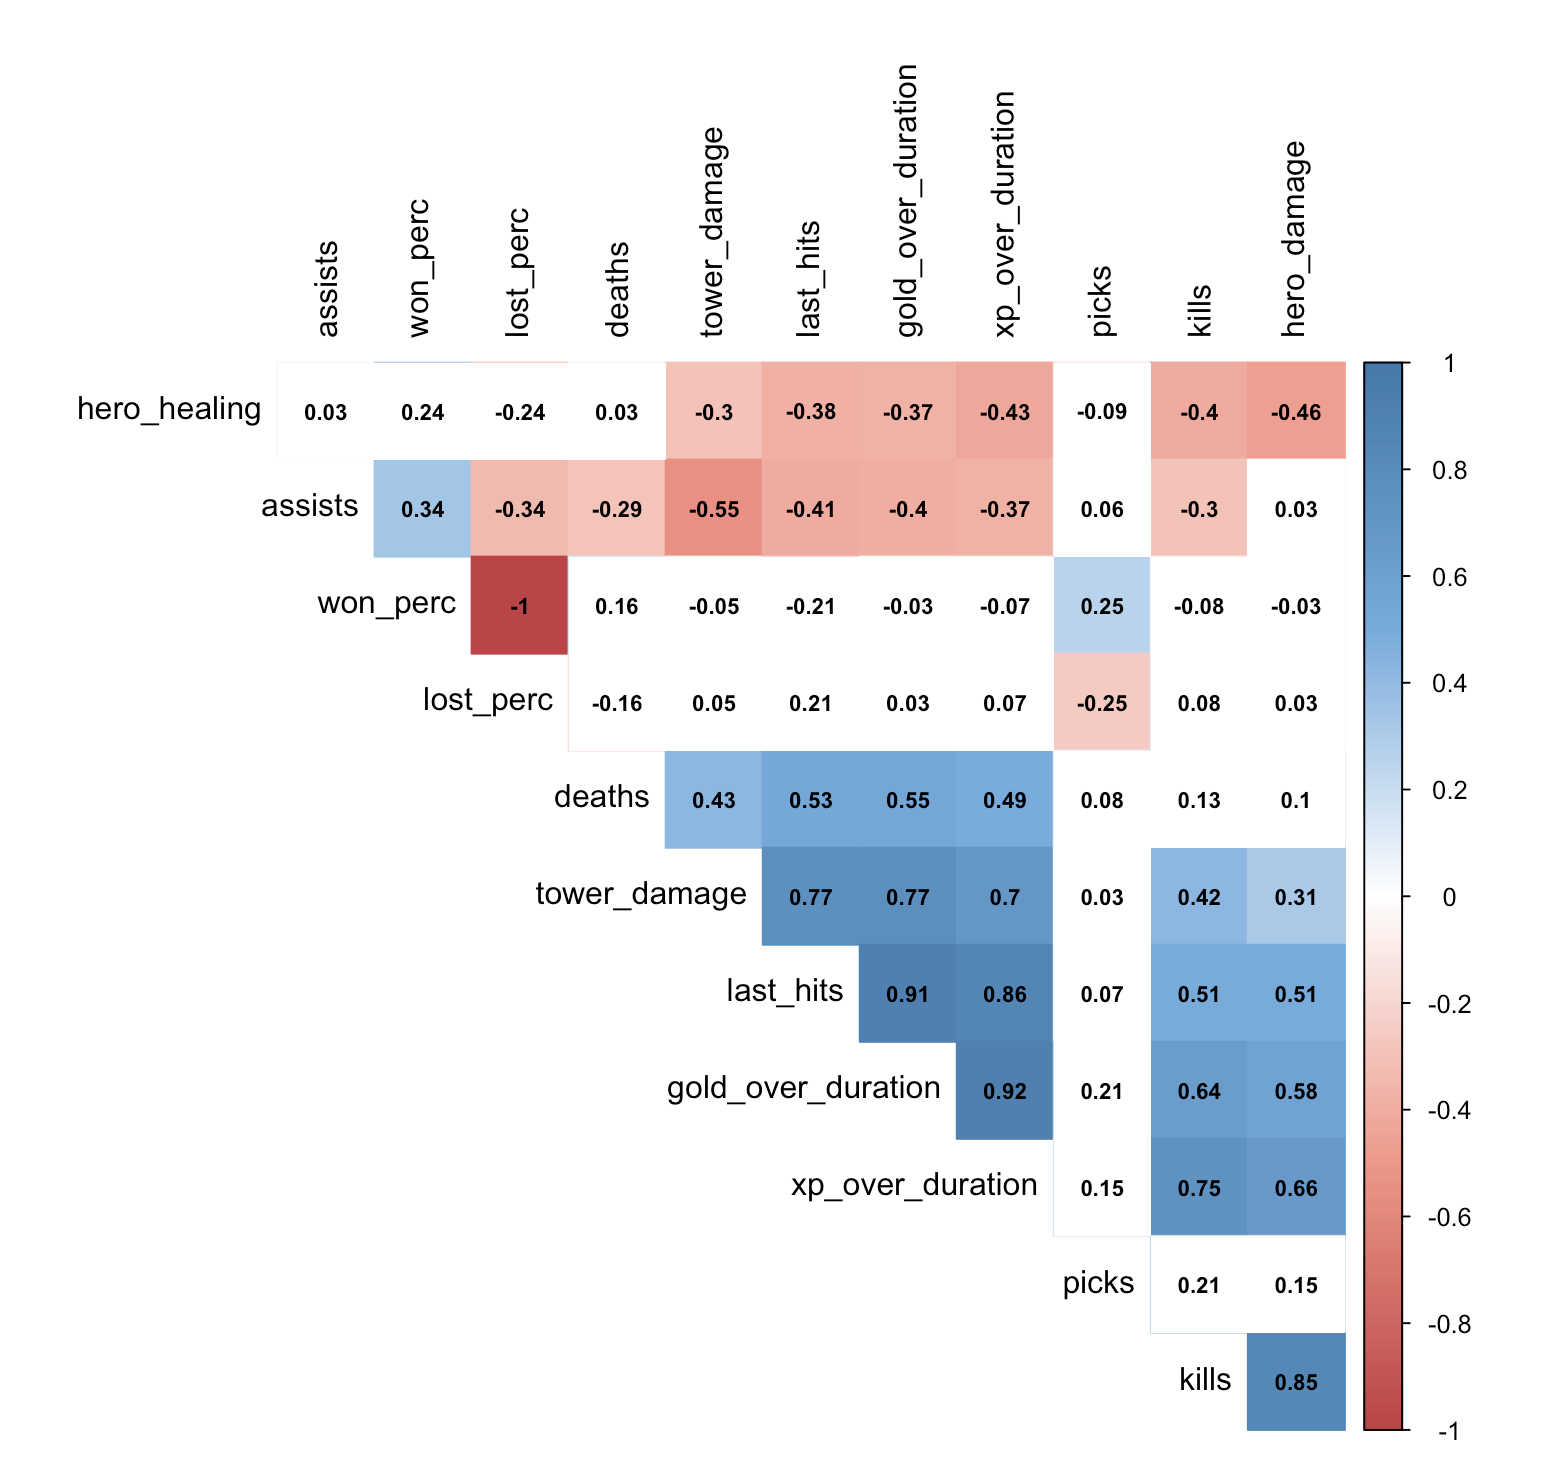
\includegraphics[width=\linewidth]{pics/corr_mat.png}
	\caption{Matrice di correlazione delle feature del dataset}
	\label{fig:cor-mat}
\end{figure}

\begin{figure}[H]
	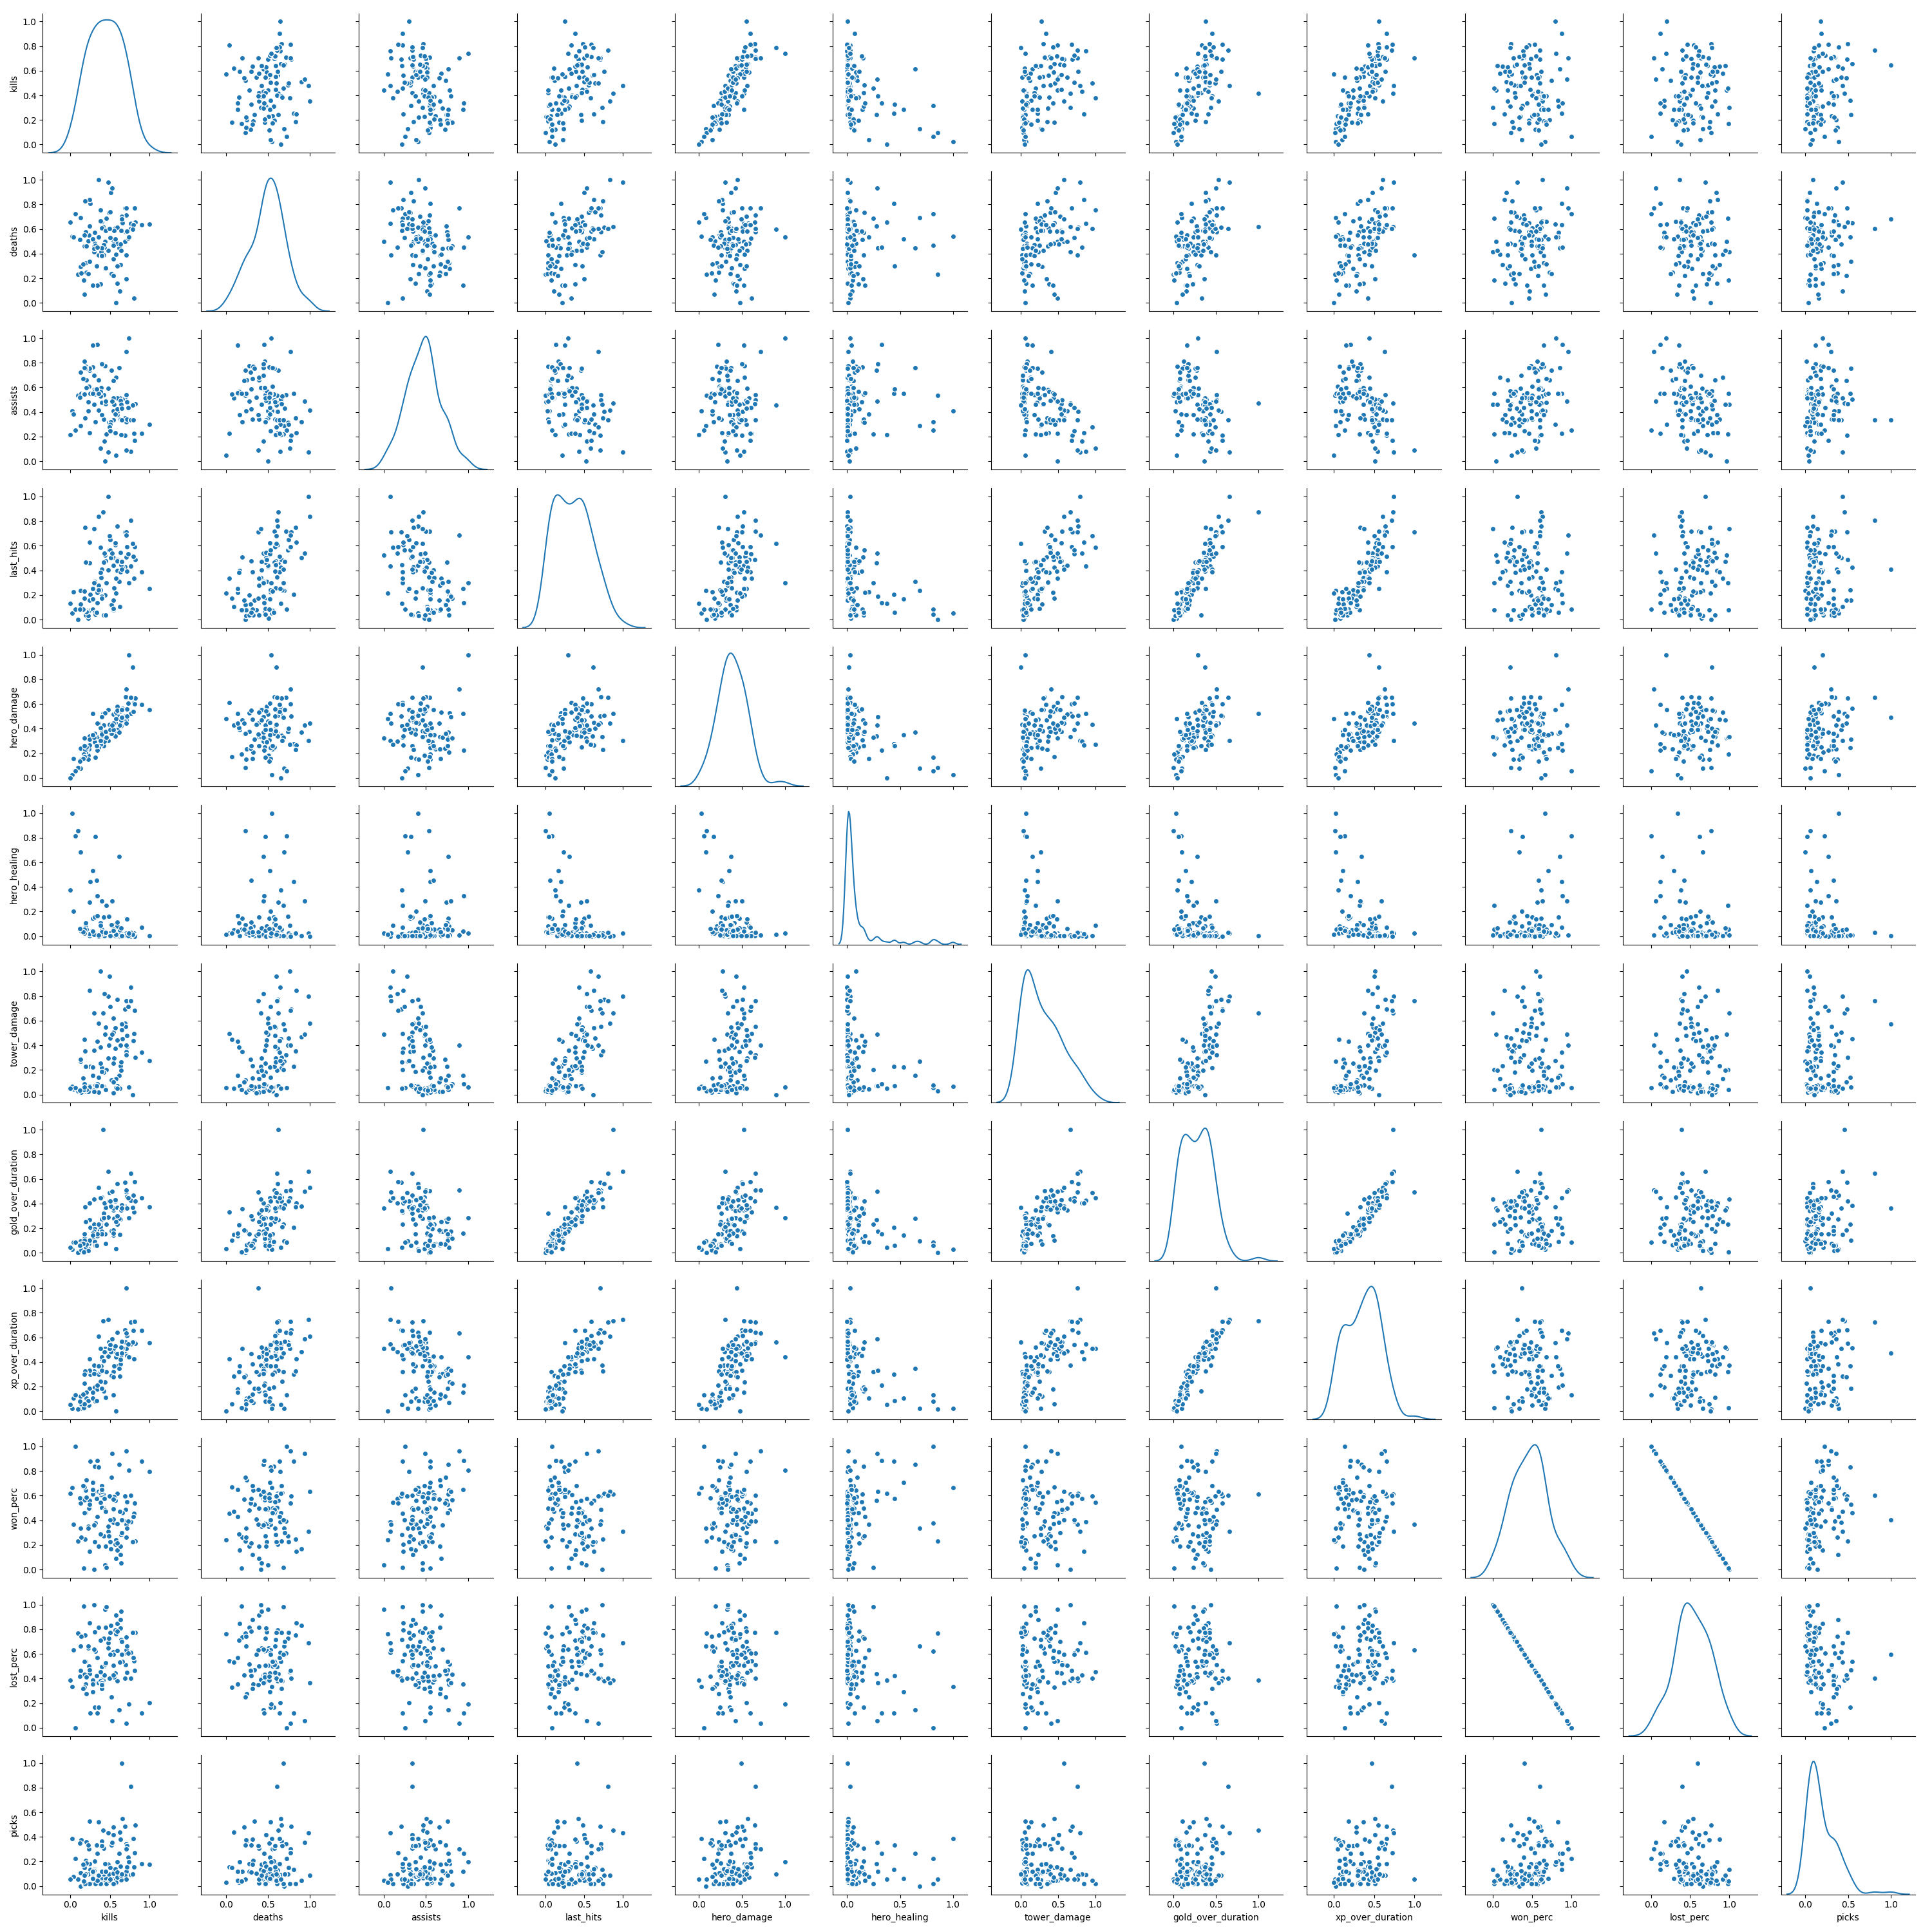
\includegraphics[width=\linewidth]{pics/pairplot.png}
	\caption{Plot delle feature a coppie}
	\label{fig:pairplot}
\end{figure}

\section{Esperimenti condotti}

\subsection{Utilizzo di tutte le feature eccetto lost\_perc}
\begin{table}[!h]
	\scriptsize	
	\centering	
	\begin{tabularx}{0.22\textwidth}{r | rrr} 
		  & 1    & 2    & 3    \\
		  \midrule
		  1 & 0    & 0,81 & 1,17 \\
		  2 & 0,81 & 0    & 0,70 \\
		  3 & 1,17 & 0,70 & 0    \\
	\end{tabularx}
	\hspace{6em}
	\begin{tabularx}{0.27\textwidth}{r | rrr} 
		  & 1    & 2    & 3    \\
		  \midrule
		  distanza & 0,28 & 0,22 & 0,25 \\
	\end{tabularx}
	\captionof{table}{Nella prima tabella la casella (i,j) rappresenta la distanza tra il centroide i e il centroide j. Nella seconda invece troviamo la somma normalizzata delle distanze di tutti i punti di un cluster dal proprio centroide}
\end{table}
Un primo esperimento è stato svolto effentuando il clustering utilizzando tutte le feature ad eccezione di \verb|lost_perc| in quanto perfettamente correlata a \verb|win_perc| essendo stata calcolata in funzione di quest'ultima. In figura \ref{fig:chooseK_3} si può osservare come il numero di cluster ottimale sia tre. Si può inoltre notare che già da quattro cluster in poi, la precisione del modello diminuisce sensibilmente per poi riamuntare leggermente solo da ventisette cluster in poi, valore eccessivamente alto soprattutto considerando le 110 istanze del dataset.\\
Il KMeans ha individuato due cluster che contengono ognuno circa il 40\% e il 50\% delle istanze, mentre il terzo cluster contiene solo il restante 10\%, come si può notare dal grafico delle silhouette in figura \ref{fig:silhouette_3}.
In figura \ref{fig:baroplot_3} si possono vedere i valori dei centroidi di ogni cluster. In particolare si può notare che il terzo cluster è caratterizzato da valori relativamente bassi per la maggior parte degli attributi ad eccezione di \verb|hero_healing| e di \verb|won_perc|.  Questo ci suggerisce che il terzo cluster contiene campioni il cui ruolo principale è quello di \textit{support}, ovvero tendono ad assistere gli altri giocatori durante i combattimenti piuttosto che a combattere contro gli avversari. Per quanto riguarda gli altri due cluster, invece, possiamo vedere una divisione in \textit{"statistiche più alte"} e \textit{"Statistiche più basse"}.\\
Dalla matrice di dissimilarità \ref{fig:diss-mat_3} possiamo notare come il primo cluster sia molto dissimile dagli altri due, entrambi caratterizzati per statistiche relativamente basse (ad eccezione di cure e vittorie).\\
Un'altra considerazione che possiamo fare è che, utilizzare dei \textit{support} favorisce il gioco di squadra e aumenta di conseguenza la percentuale di vittorie.

\begin{figure}[H]
	\centering
	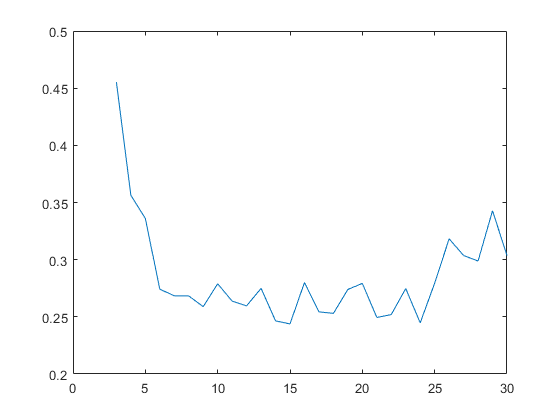
\includegraphics[width=0.8\linewidth]{pics/no11/chooseK.png}
	\caption{Silhouette media al variare del numero di cluster utilizzando tutte le feature tranne lost\_perc}
	\label{fig:chooseK_3}
\end{figure}
\begin{figure}[H]
	\centering
	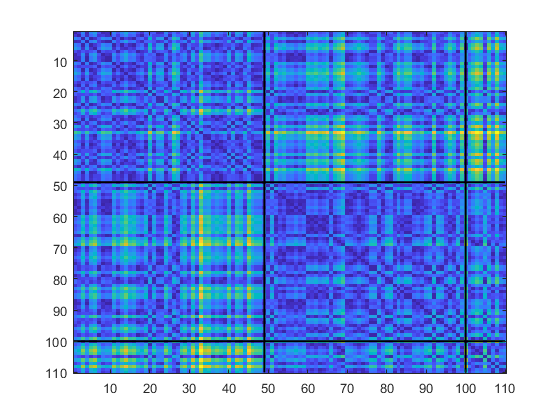
\includegraphics[width=0.8\linewidth]{pics/no11/diss_mat.png}
	\caption{Matrice di dissimilarità del clustering ottimo utilizzando tutte le feature tranne lost\_perc}
	\label{fig:diss-mat_3}
\end{figure}
\begin{figure}[H]
	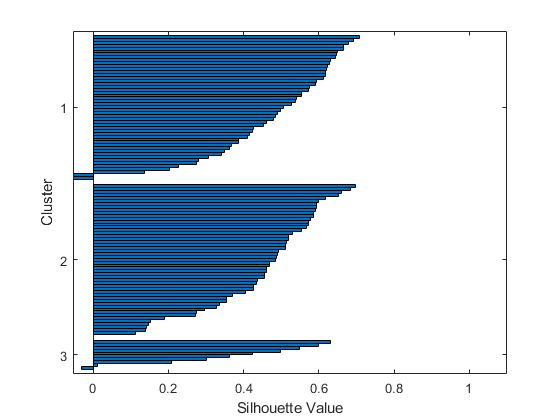
\includegraphics[width=\linewidth]{pics/no11/silhouette.png}
	\caption{Silhouette del clustering ottimo utilizzando tutte le feature tranne lost\_perc}
	\label{fig:silhouette_3}
\end{figure}
\begin{figure}[H]
	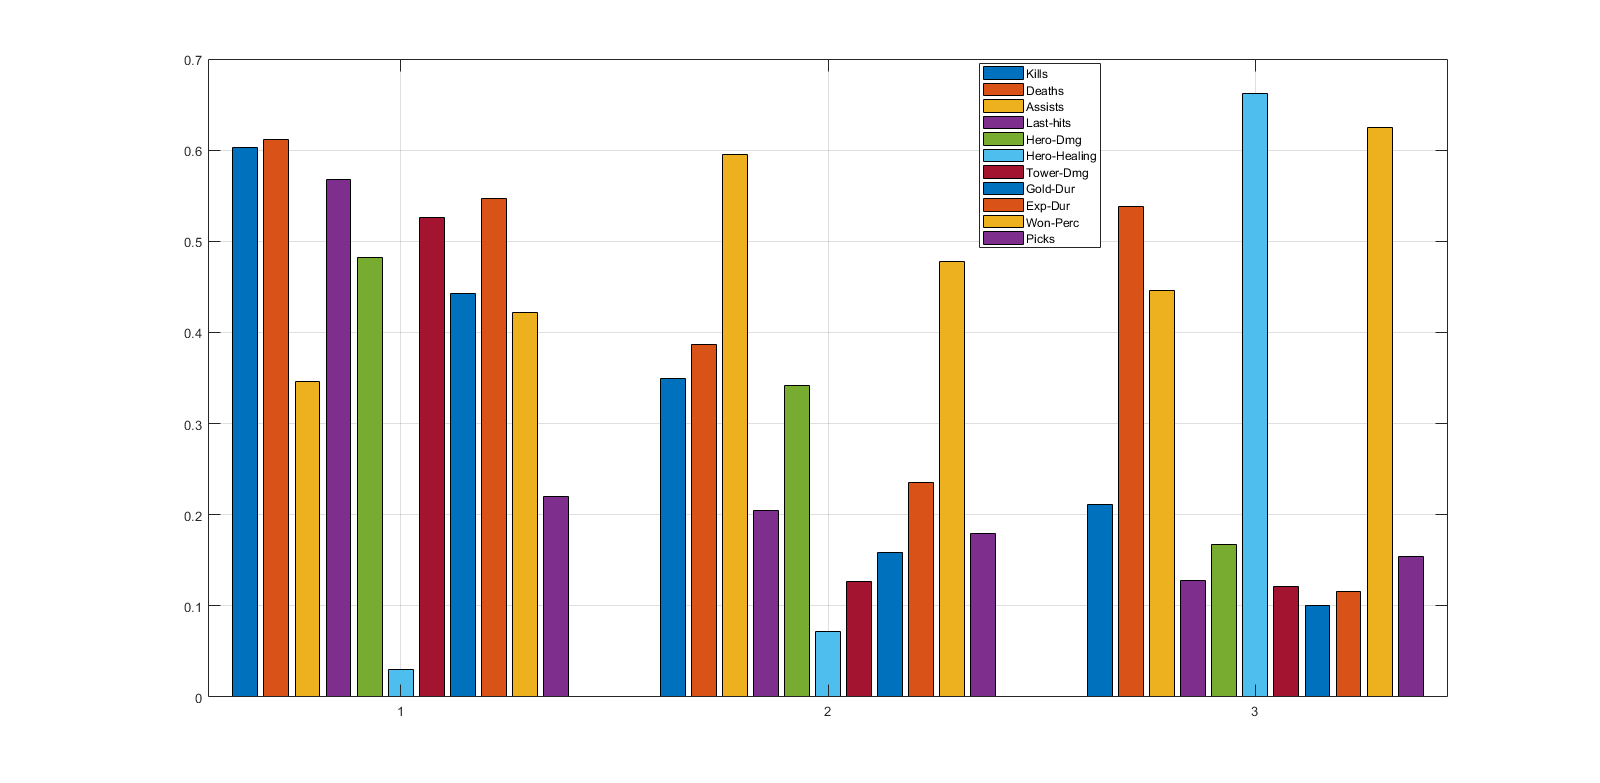
\includegraphics[width=\linewidth]{pics/no11/barplot.png}
	\caption{Barplot delle istanze clusterizzate utilizzando tutte le feature tranne lost\_perc}
	\label{fig:baroplot_3}
\end{figure}


\subsection{Utilizzo di tutte le feature eccetto gold\_over\_duration e lost\_perc}
\begin{table}[!h]
	\scriptsize	
	\centering	
	\begin{tabularx}{0.22\textwidth}{r | rrr} 
		& 1    & 2    & 3    \\
		\midrule
		1 & 0    & 0,70 & 0,77 \\
		2 & 0,70 & 0    & 1,12 \\
		3 & 0,77 & 1,12 & 0    \\
	\end{tabularx}
	\hspace{6em}
	\begin{tabularx}{0.27\textwidth}{r | rrr} 
         & 1    & 2    & 3    \\
         \midrule
         distanza & 0,22 & 0,25 & 0,27 \\
	\end{tabularx}
	\captionof{table}{Nella prima tabella la casella (i,j) rappresenta la distanza tra il centroide i e il centroide j. Nella seconda invece troviamo la somma normalizzata delle distanze di tutti i punti di un cluster dal proprio centroide}
\end{table}
Il secondo esperimento è stato svolto eliminando anche \verb|gold_over_duration|, oltre a \verb|lost_perc| in quanto correlata sia a \verb|xp_over_duration| che alla somma di \verb|kills| e \verb|last_hits| (il modo più efficace di guadagnare monete è infatti uccidendo i campioni avversari e i \textit{creeps}).\\
Rimuovendo due feature il numero di cluster ottimo rimane di tre, ma si si può notare che la precisione della clusterizzazione con quattro e cinque gruppi è aumentata sensibilmente mentre rimane bassa per clusterizzazioni con più di cinque gruppi.\\
Rispetto alla clusterizzazione precedente, come si può notare sia dalla silhouette \ref{fig:silhouette_2} e dal barplot in figura \ref{fig:baroplot_2}, non ci sono grosse differenze e continua ad essere identificato il gruppo dei \textit{support} con circa il 10\% delle istanze.\\
Analoghe considerazioni possono essere fatte per la matrice di dissimilarità.

\begin{figure}[H]
	\centering
	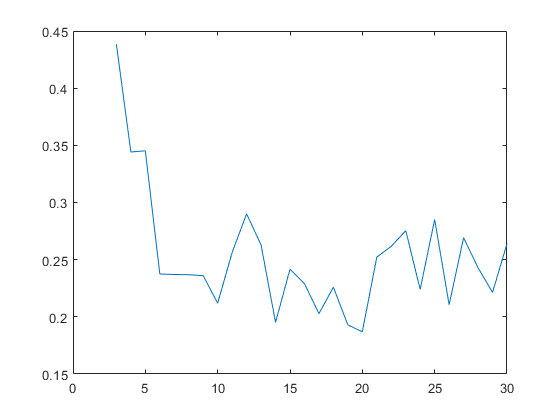
\includegraphics[width=0.8\linewidth]{pics/no8_11/chooseK.png}
	\caption{Silhouette media al variare del numero di cluster utilizzando tutte le feature tranne gold\_over\_duration e lost\_perc}
	\label{fig:chooseK_2}
\end{figure}
\begin{figure}[H]
	\centering
	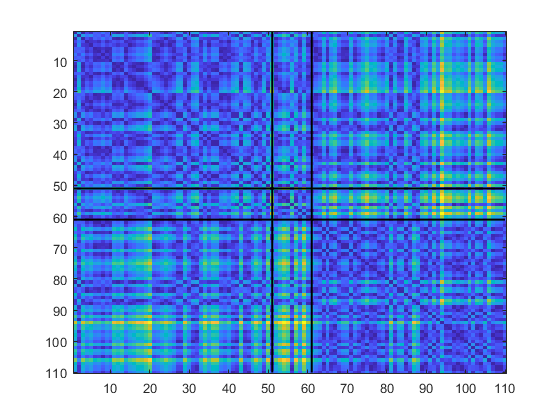
\includegraphics[width=0.8\linewidth]{pics/no8_11/diss_mat.png}
	\caption{Matrice di dissimilarità del clustering ottimo utilizzando tutte le feature tranne gold\_over\_duration e lost\_perc}
	\label{fig:diss-mat_2}
\end{figure}
\begin{figure}[H]
	\centering
	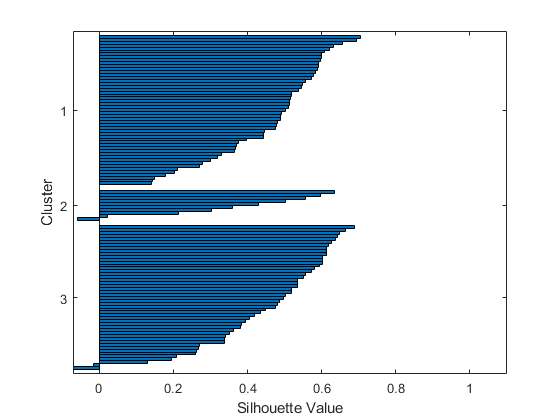
\includegraphics[width=0.9\linewidth]{pics/no8_11/silhouette.png}
	\caption{Silhouette del clustering ottimo utilizzando tutte le feature tranne gold\_over\_duration e lost\_perc}
	\label{fig:silhouette_2}
\end{figure}
\begin{figure}[H]
	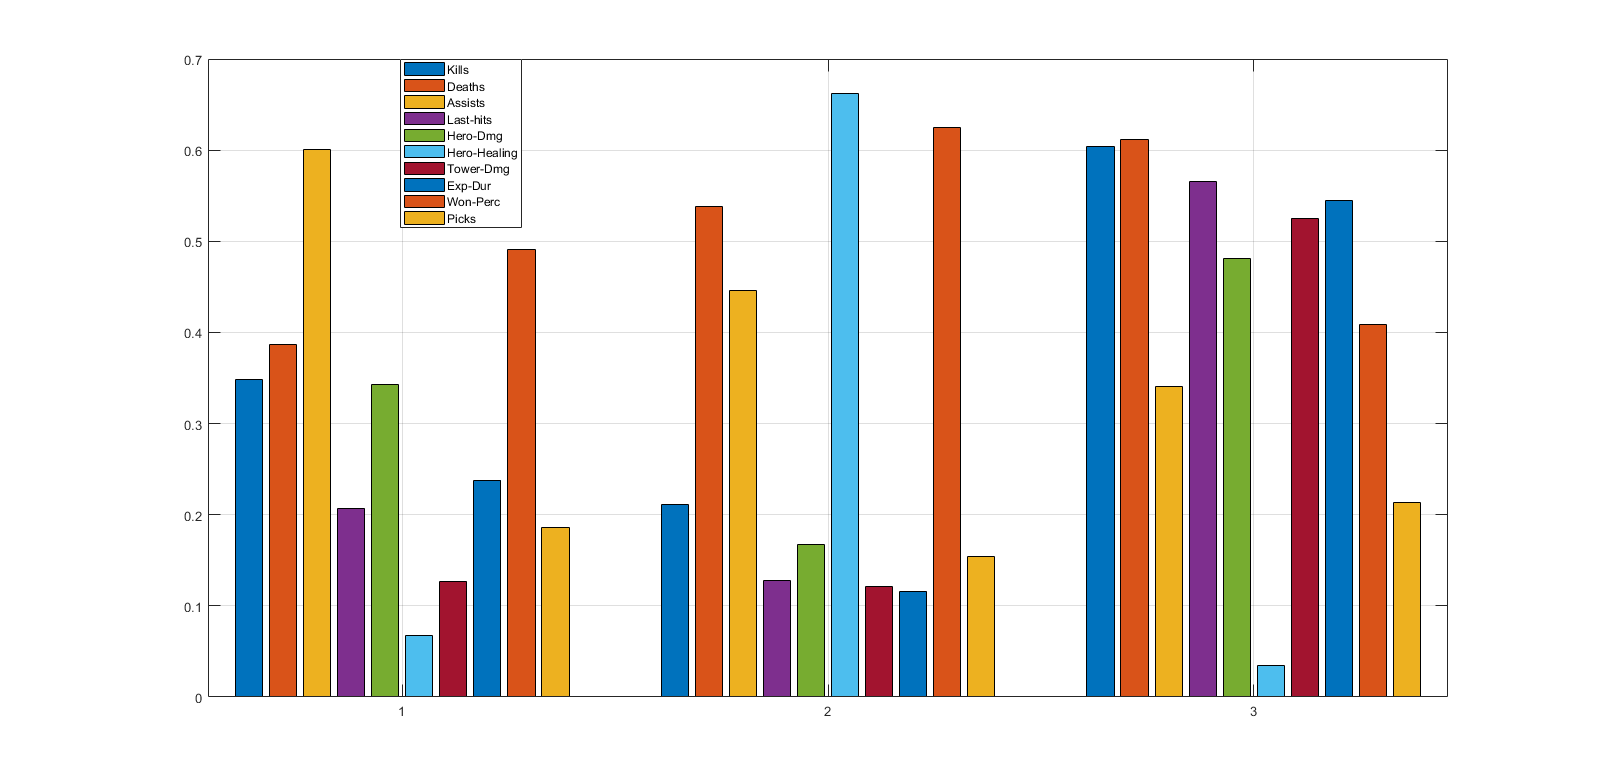
\includegraphics[width=\linewidth]{pics/no8_11/barplot.png}
	\caption{Barplot delle istanze clusterizzate utilizzando tutte le feature tranne gold\_over\_duration e lost\_perc}
	\label{fig:baroplot_2}
\end{figure}



\subsection{Utilizzo delle prime sette feature}
\begin{table}[!h]
	\scriptsize	
	\centering	
	\begin{tabularx}{0.27\textwidth}{r | rrrr} 
		& 1    & 2    & 3    & 4    \\
		\midrule
		1 & 0,00 & 0,94 & 0,56 & 0,50 \\
		2 & 0,94 & 0,00 & 0,68 & 1,07 \\
		3 & 0,56 & 0,68 & 0,00 & 0,84 \\
		4 & 0,50 & 1,07 & 0,84 & 0,00 \\
	\end{tabularx}
	\hspace{6em}
	\begin{tabularx}{0.32\textwidth}{r | rrrr} 
         & 1    & 2    & 3   & 4	\\
         \midrule
         distanza & 0,15 & 0,16 & 0,1 & 0,13 \\
	\end{tabularx}
	\captionof{table}{Nella prima tabella la casella (i,j) rappresenta la distanza tra il centroide i e il centroide j. Nella seconda invece troviamo la somma normalizzata delle distanze di tutti i punti di un cluster dal proprio centroide}
\end{table}
Un'altro esperimento è stato fatto utilizzando le sole prime sette feature, ovvero escludendo le feature che rappresentano i risultati delle partite o le preferenze dei giocatori. Le sette feature utilizzate sono: \verb|kills, deaths, assists, last_hits, hero_damage,| \verb|hero_healing, tower_damage|.
La prima cosa che possiamo notare (figura \ref{fig:chooseK_1}) è che in questo caso, il numero di cluster ottimo è aumentato a quattro, anche se si continua ad avere un buon raggruppamento utilizzando tre cluster.\\
Analizzando i valori dei centroidi riportati in figura \ref{fig:baroplot_1} possiamo notare che ancora una volta viene identificato il cluster dei \textit{support}, mentre quello che prima era il cluster caratterizzato da statistiche più alte è stato diviso in due cluster di dimensione minore. In questi due cluster potremmo identificare due categorie di campioni, gli \textit{split pusher} e i \textit{carry}, i primi caratterizzati da elevati danni alle torri, e i secondi da danni ed uccisioni elevati.\\
Dalla matrice di dissimilarità in figura \ref{fig:diss-mat_1} possiamo notare che i cluster 1 e 4 in cui abbiamo identificato \textit{carry} e \textit{split pusher} si presentano piuttosto simili, così come i cluster 2 e 3.

\begin{figure}[H]
	\centering
	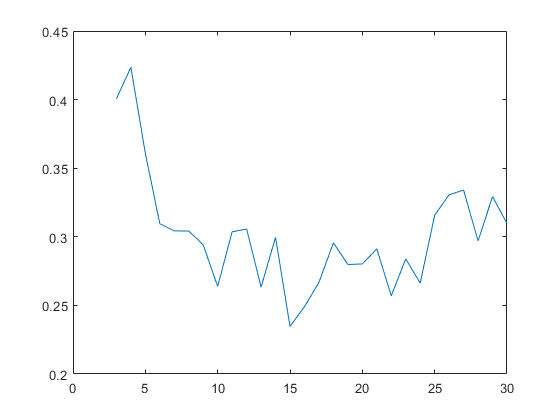
\includegraphics[width=0.8\linewidth]{pics/1to7/chooseK.png}
	\caption{Silhouette media al variare del numero di cluster ottimo utilizzando le prime sette feature}
	\label{fig:chooseK_1}
\end{figure}
\begin{figure}[H]
	\centering
	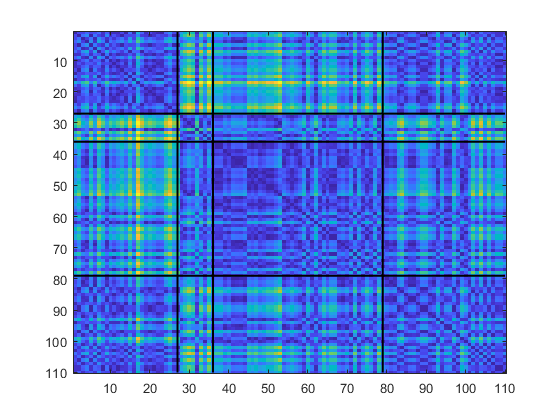
\includegraphics[width=0.8\linewidth]{pics/1to7/diss_mat.png}
	\caption{Matrice di dissimilarità del clustering ottimo utilizzando le prime sette feature}
	\label{fig:diss-mat_1}
\end{figure}
\begin{figure}[H]
	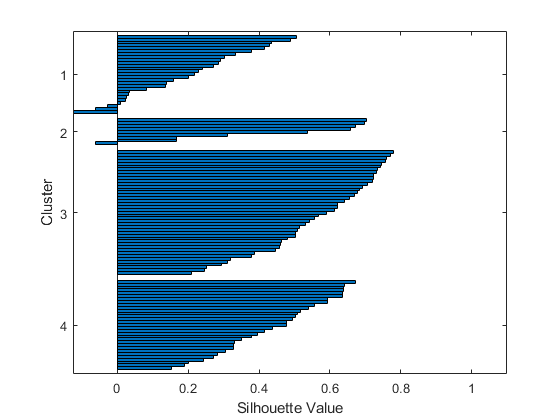
\includegraphics[width=\linewidth]{pics/1to7/silhouette.png}
	\caption{Silhouette del clustering ottimo utilizzando le prime sette feature}
	\label{fig:silhouette_1}
\end{figure}
\begin{figure}[H]
	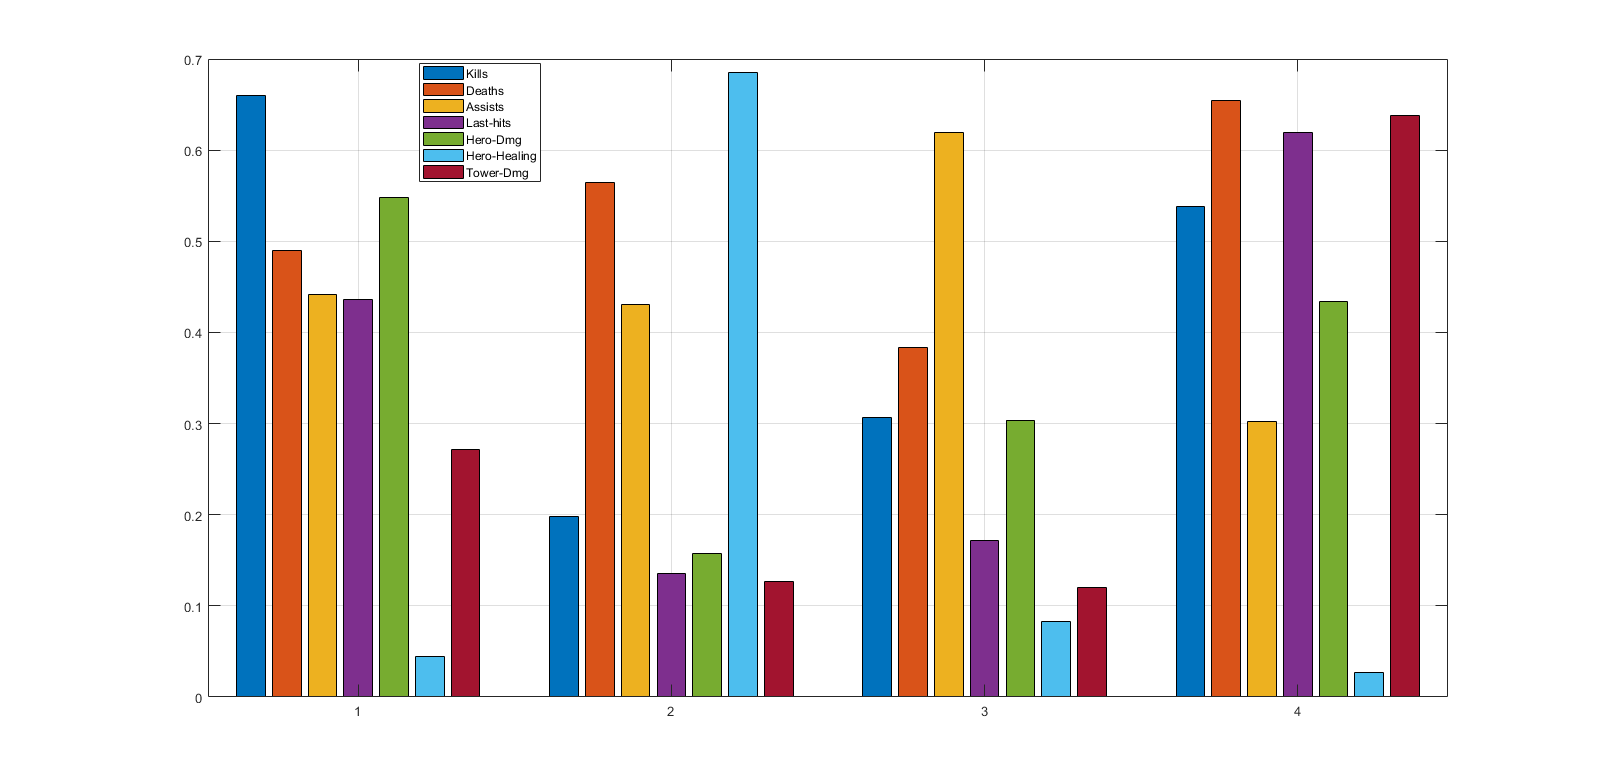
\includegraphics[width=\linewidth]{pics/1to7/barplot.png}
	\caption{Barplot delle istanze clusterizzate utilizzando le prime sette feature}
	\label{fig:baroplot_1}
\end{figure}



\subsection{Utilizzo delle prime sette feature e cinque cluster}
Spinti dalle osservazioni precedenti riguardo le caratteristiche dei cluster, abbiamo provato ad effettuare un ultimo esperimento utilizzando le stesse feature di quello precedente, ma partizionando in cinque gruppi in cui vogliamo provare ad identificare i ruoli principali in cui può giocare un personaggio.\\
Analizzando i centroidi ottenuti (figura \ref{fig:clustering-roles}) possiamo provare ad ipotizzare ed associare un ruolo ad ogni cluster. Come per gli esperimenti precedenti è facile identificare nel quinto cluster la categoria dei \textit{support}, caratterizzati da cure elevate e dal resto delle statistiche relativamente basso. Analogamento il quattro e il secondo cluster possiamo associarli rispettivamente ai \textit{carry} e agli \textit{split pusher}. Per quanto riguarda il terzo cluster possiamo notare che è caratterizzato da un elevato numero di assist e valori particolarmente bassi per il resto delle statistiche. Questo ci porta ad associare al terzo cluster la categoria dei \textit{tank} ovvero quei campioni che non spiccano per danni inflitti, ma caratterizzati da elevata resistenza ai danni che li rende particlarmente adatti ad essere utilizzati come bersaglio e per iniziare i combattimenti (questo porta a giustificare il numero di assist elevato). Per questo cluster ci saremmo aspettati però un maggior numero di morti. Infine abbiamo il primo cluster caratterizzato da valori nella media per tutte le feature ad eccezione delle cure. Avendo statistiche nella media è difficile associare un unico ruolo a questa categoria e abbiamo deciso di associare \textit{fighter} (guerrieri da mischia con statistiche nella media) e \textit{assassini} (personaggi particolarmente vulnerabili ma in grado di effettuare moltissimi danni in poco tempo).\\\\
Fatte queste considerazioni, abbiamo assegnato manualmente ad ogni campione una label con il suo ruolo effettivo e ad ogni cluster il ruolo corrispondete in modo da poter verificare la correttezza del clustering. Su 110 campioni, 72 sono stati assegnati al cluster corretto raggiungendo quindi un'accuratezza del 65\%.
\begin{table}[!h]
	\scriptsize	
	\centering
	\begin{tabularx}{0.33\textwidth}{lr} 
		hero\_name  &    heroclass \\ 
		\midrule
		Abaddon  &      Support \\
		Alchemist  & Split Pusher \\
		Ancient Apparition  &         Tank \\
		Anti-Mage  & Split Pusher \\
		Axe  &      Fighter / Assassin \\
		Bane  &         Tank \\
		Batrider  &         Tank \\
		Beastmaster  &         Tank \\
		Bloodseeker  &      Fighter / Assassin \\
		Bounty Hunter  &         Tank \\
	\end{tabularx}
	\captionof{table}{Classe associata ad ogni campione}
\end{table}

\begin{figure}
	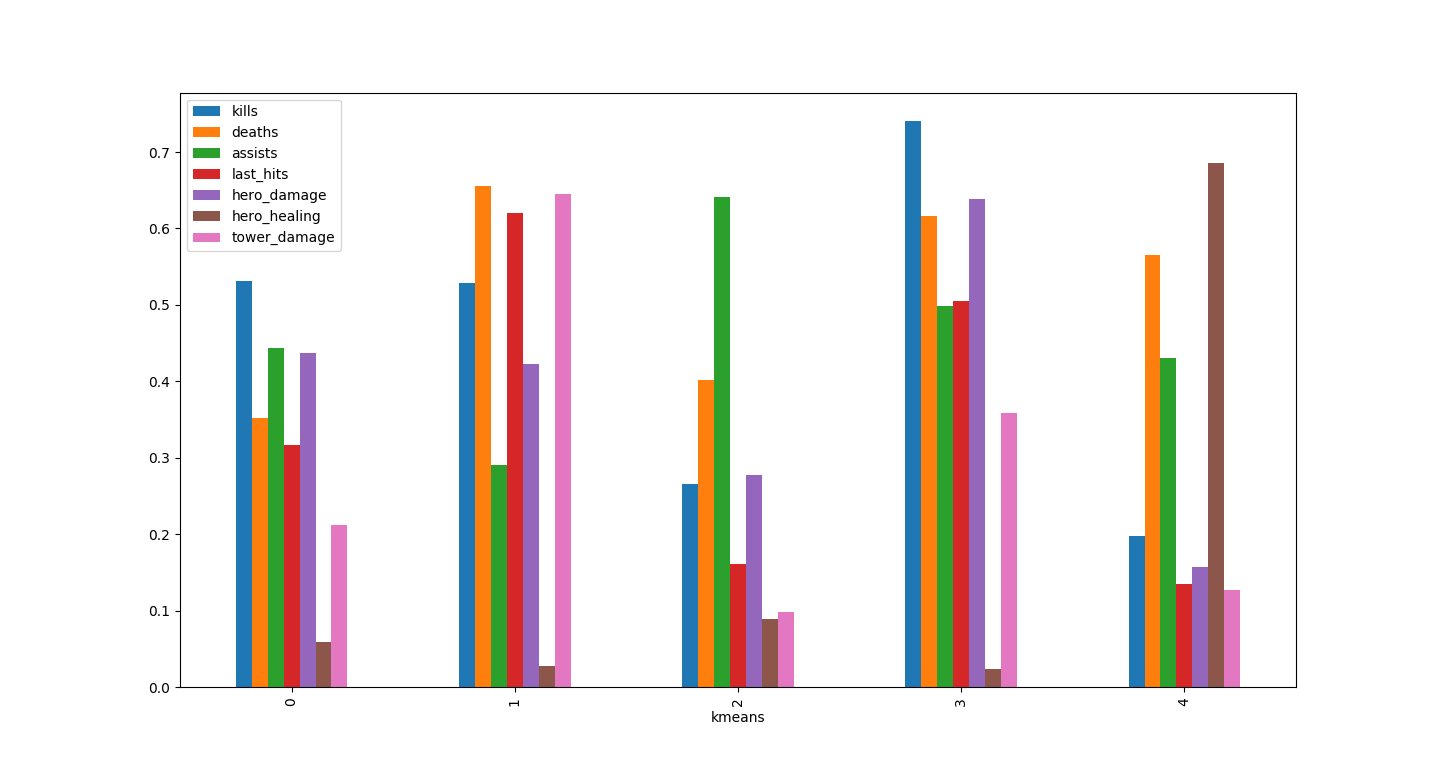
\includegraphics[width=\linewidth]{pics/clustering_roles.png}
	\caption{Centroidi dopo aver clusterizzato in cinque cluster}
	\label{fig:clustering-roles}
\end{figure}

\begin{figure}
	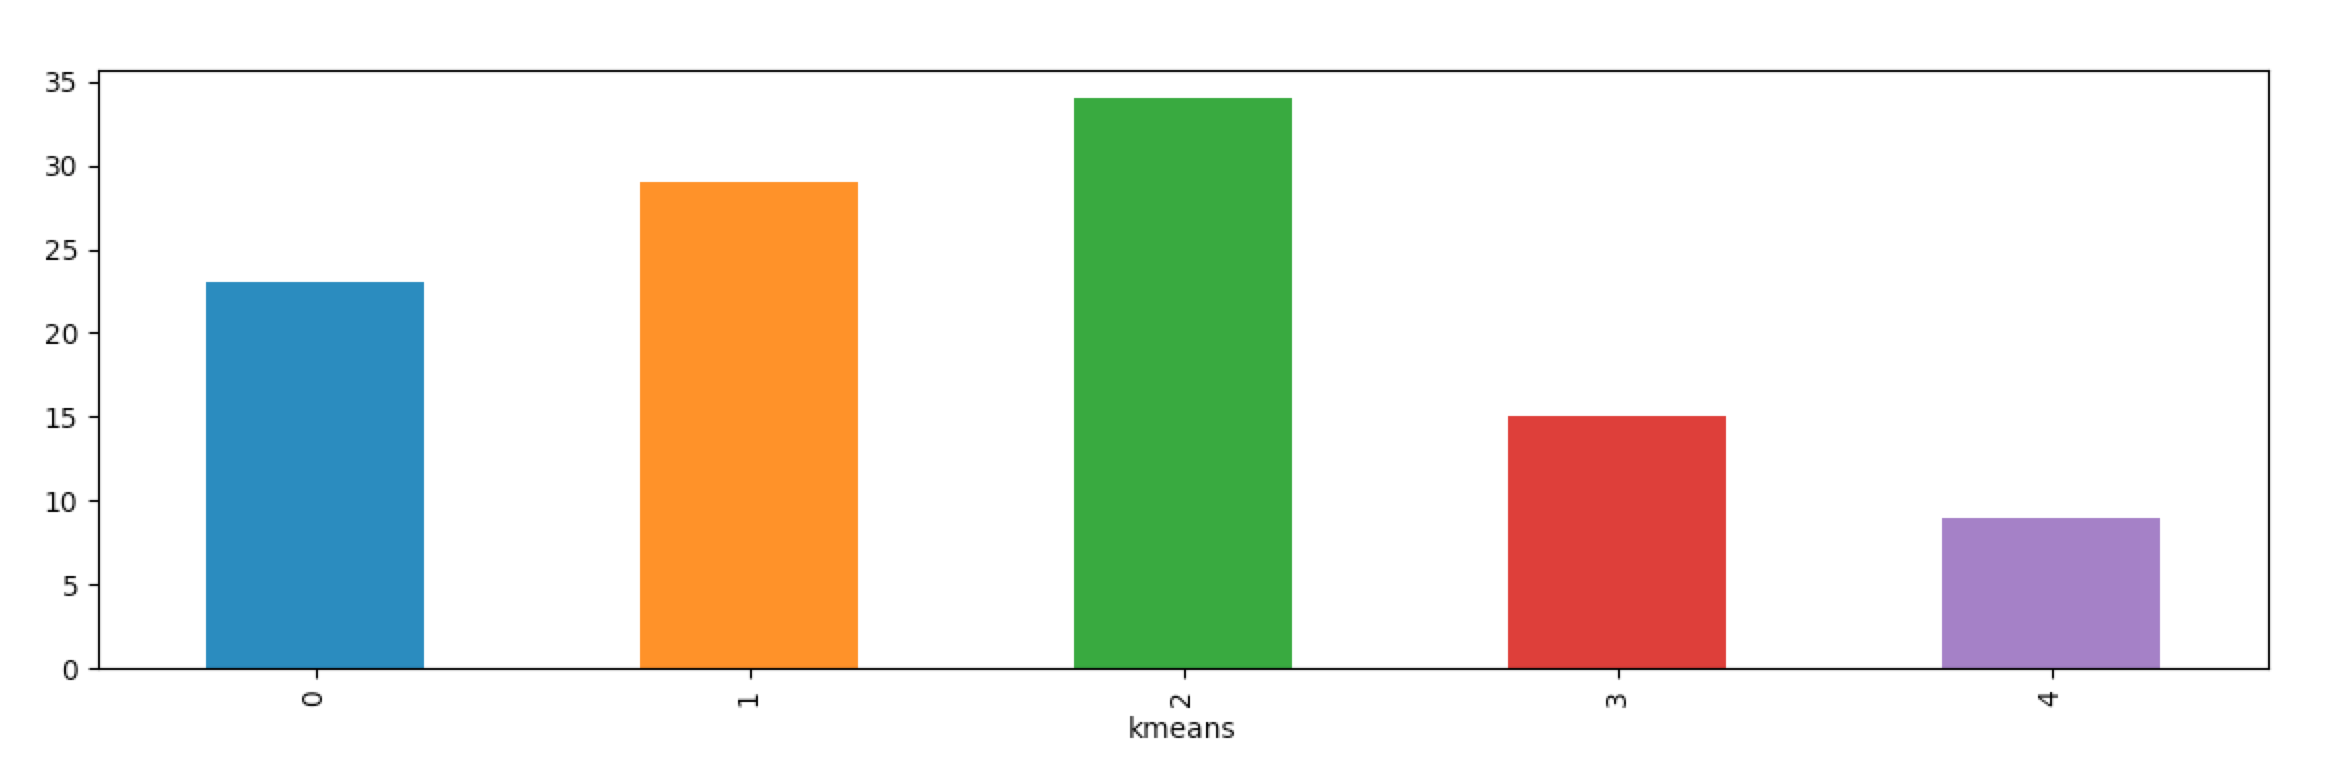
\includegraphics[width=\linewidth]{pics/clustering_roles_n.png}
	\caption{Numero di istanze in ogni cluster}
	\label{fig:clustering-roles-n}
\end{figure}

\begin{figure}[H]
	\centering
	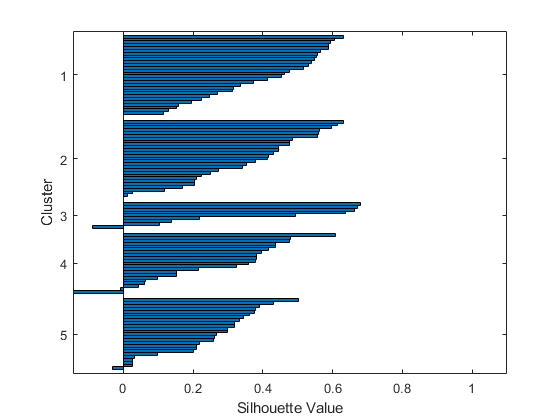
\includegraphics[width=0.8\linewidth]{pics/silhouette.png}
	\caption{Silhouette del clustering utilizzando le prime sette feature e cinque cluster}
	\label{fig:silhouette}
\end{figure}

\begin{figure}[H]
	\centering
	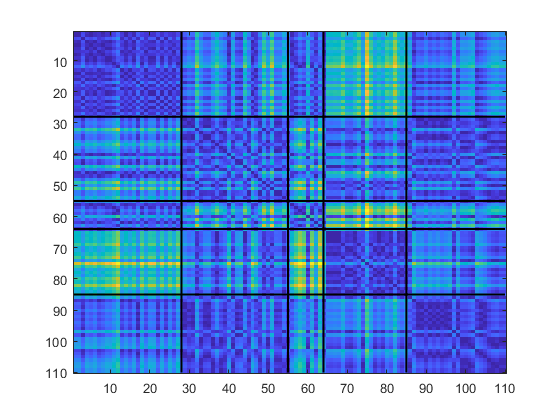
\includegraphics[width=0.8\linewidth]{pics/diss_mat.png}
	\caption{Matrice di dissimilarità del clustering utilizzando le prime sette feature e cinque cluster}
	\label{fig:diss-mat}
\end{figure}



\chapter{Conclusioni}
In questa relazione abbiamo descritto il processo di integrazione di tre dataset riguardanti i risultati di partita al videogame \textit{DOTA 2} per poi applicare delle tecniche di clustering utilizzando l'algoritmo \textit{K-Means}. Per quanto riguarda la parte di Data Technology abbiamo descritto il processo di integrazione dei dataset e analizzato due diverse dimensioni di qualità, sia prima che dopo il processo di integrazione, discutendo e motivando le scelte prese al fine di migliorare la qualità del dataset. Abbiamo poi effettuato delle analisi descrittive sia sui dati a disposizione prima del processo di integrazione, sia su quelli integrati e abbiamo cercato eventuali relazioni tra campioni, squadre e durate delle partite.
\\[0.8em]
Per quanto riguarda la parte di Machine Learning abbiamo cercato eventuali correlazioni sulle feature a disposizione in modo da utilizzare solo quelle di maggior interesse e di ottenere una classificazione migliore. Abbiamo poi effetuato quattro esperimenti di clustering utilizzando l'algoritmo \textit{K-Means} utilizzando diversi sottoinsiemi di feature. Inizialmente pensavamo di ottenere dei cluster che rispecchiassero la forza dei campioni, ma, come descritto nelle osservazioni dei primi tre esperimenti condotti, il raggruppamento sembrava avvenire in base al loro ruolo. Per questo motivo abbiamo deciso di condurre un quarto ed ultimo esperimento imponendo l'uso di cinque cluster per validare la nostra ipotesi. Abbiamo poi assegnato manualmente delle label ad ogni personaggio associandogli i suoi ruoli effettivi in modo da confrontarli con la clusterizzazione ottenendo una percentuale di correttezza del 65\%.

\end{document}





%%%% end of file -- test-draft.tex
